\documentclass[12pt]{article}

\usepackage[utf8]{inputenc}
\usepackage[T1]{fontenc}
\usepackage{color}
\usepackage[hyphens]{url}
\usepackage{enumitem}
\usepackage{amsmath}
\usepackage{amsfonts}
\usepackage{geometry}
\usepackage{graphicx}
\usepackage{cite}
\usepackage[unicode,hidelinks]{hyperref}
\usepackage{tocloft}
\usepackage{array}
\usepackage{titlesec}
\usepackage{caption}
\usepackage{xcolor}

\newcommand{\vek}[1]{\overrightarrow{#1}}
\newcommand{\ocena}[1]{\textcolor{red}{#1}}
\renewcommand{\refname}{Literatura}
\renewcommand{\contentsname}{Sadržaj}
\renewcommand{\cftsecfont}{\bfseries}
\renewcommand{\cftsecpagefont}{\bfseries}
\setlength{\cftbeforesecskip}{0.5cm}
\setlength{\cftsecindent}{0pt}
\setlength{\cftsubsecindent}{1.5cm}
\geometry{top=1in, bottom=1in, left=1in, right=1in}
\hypersetup{colorlinks,citecolor=green,filecolor=green,linkcolor=blue,
urlcolor=blue}
\setlength{\parskip}{0.1cm}


\begin{document}

\begin{titlepage}

    \newcommand{\HRule}{\rule{\linewidth}{0.4mm}}
    \center
    \textsc{\LARGE Matematički fakultet}\\[5cm]

    \HRule\\[0.4cm]
    {\LARGE\bfseries Skica odgovora na teorijska ispitna pitanja iz geometrije kod profesora
    Srđana Vukmirovića}
    \\[0.2cm]
    \HRule\\
    {\large\bfseries Za potpuno razumevanje i potpune odgovore je potrebno pogledati
    knjigu ,,Geometrija za informatičare`` (link do knjige je ostavljen u odeljku \hyperref[literatura]{literatura})}
    \\[0.2cm]

    \vspace{16\baselineskip}
    \begin{flushleft}
        \large
        \textit{Radio}\\
        Lazar Jovanović 34/2023
    \end{flushleft}

    \vfill\vfill\vfill\vfill
    {\large Beograd, 2024/2025}
    \vfill

\end{titlepage}

\tableofcontents
\newpage

\section{Konvencije}
\textit{Sve konvencije važe dok se ne naglasi drugačije.}
\par
\vspace*{1cm}

\textbf{Primeri i slike:} Većina primera i slika neće biti navedena.

\textbf{Množenje i skalarni proizvod:} Množenje broja i vektora se neće označavati posebnom
oznakom, dok će se za skalarni proizvod koristiti oznaka $\cdot$.
\par

\textbf{Uglovi:} Uglovi između vektora će se označavati sa
$\angle{\vek{v}\vek{u}}$, a uglovi formirani od tri tačke sa $\angle{ABC}$ gde
će se posmatrati ugao kod tačke $B$. Podrazumeva se da se posmatra ugao u
pozitivnom smeru od $\vek{v}$ do $\vek{u}$, odnosno, od $AB$ do $BC$. Ugao je
iz intervala $[0,2\pi)$.
\par

\textbf{Oznaka vektora:} Ako posmatramo vektore, onda ih označavamo sa
$\vek{u}$. Ako posmatramo samo kolone koordinata vektora, onda ih označavamo sa
$u$.
\par

\textbf{Mase tačaka:} Za tačku $A$ oznaka $A(m_A)$ znači da tačka $A$ ima
dodeljenu masu $m_A$. Podrazumevaće se da se i bez navedene oznake oznaka
$m_{A}$ odnosi na tačku $A$.
\par

\textbf{Baza vektorskog prostora:} Označavamo $i$-ti vektori baze $e$ sa
$\vek{e_i}$.
\par

\textbf{Ortonormirana baza:} U nastavku će se ,,ortonormirane baze`` skraćeno
nazivati ,,ON baze``.
\par

\textbf{Ortonormirana baza pozitivne orijentacije:} U nastavku će se
,,ortonormirane baze pozitivne orijentacije`` skraćeno nazivati ,,ON+ baze``.
\par

\textbf{Označavanje duži:} Dužina duži koju formiraju tačke $A$ i $B$
se označava sa AB.

\newpage

\section{Pitanja}
\subsection{Vektori i osnovne operacije sa vektorima}
\textit{Sabiranje i množenje skalarom, nula vektor, suprotan vektor, kolinearni
    i komplanarni vektori, jedinični vektor, \ocena{Dokaz T1.1 (tvrđenja S1-S4)}.}
\par
\vspace*{1cm}

\textbf{Definicija vektora:} Klasa ekvivalencije usmerenih duži koje imaju isti
pravac, smer i intenzitet.
\par

\textbf{Predstavnik vektora:} Ako je usmerena duž $\vek{AB}$ predstavnik vektora
$\vek{v}$, tada pišemo $\vek{v}=\vek{AB}$.
\par

\textbf{Sabiranje vektora}: Pri sabiranju se vektori nadovezuju, posmatraju se
samo početna i krajnja tačka.
\par

\textbf{Množenje vektora skalarom:} Vektor $\alpha\vek{v}$ ima isti pravac
kao $\vek{v}$, ima intenzitet $|\alpha||\vek{v}|$ i ima isti smer ako je
$\alpha>0$, a različit smer ako je $\alpha<0$. Specijalno, ako je $\alpha=0$,
svaki vektor $\vek{v}$ postaje nula vektor.
\par

\textbf{Nula vektor:} Vektor $\vek{v}$ je nula vektor (zapisujemo kao $\vek{0}$
ili $\vek{AA}$) ako je njegov intenzitet jednak nuli. Nula vektor nema ni
pravac ni smer.
\par

\textbf{Suprotni vektor:} Suprotni vektor vektora $\vek{v}$ (zapisujemo sa
$-\vek{v}$) ima isti intenzitet i pravac kao vektor $\vek{v}$, a suprotan smer.
Takođe, suprotan vektor vektora $\vek{AB}$ možemo da zapišemo i kao $\vek{BA}$
\par

\textbf{Kolinearni vektori:} Vektori su kolinearni ako postoje njihovi predstavnici
koji pripadaju istoj pravoj.
\par

\textbf{Komplanarni vektori:} Vektori su komplanarni ako postoje njihovi predstavnici
koji pripadaju istoj ravni.
\par

\textbf{Jedinični vektor:} Vektor čiji je intenzitet $1$. Od svakog ne-nula
vektora možemo da napravimo jedinični vektor normalizacijom.
\par

\textbf{Normalizacija vektora:} Normalizacijom se od vektora $\vek{v}$ dobija
jedinični vektor $\frac{1}{|\vek{v}|}\vek{v}$. Ovaj vektor ima isti pravac
i smer kao početni vektor, a intenzitet mu je $1$.
\par

\textbf{T1.1:} Neka su $\vek{u}, \vek{v}, \vek{w}\in\mathbb{V}$. Tada važe
sledeća tvrđenja:
\begin{enumerate}[label=\textbf{(S\arabic*)}]
    \item $(\vek{u}+\vek{v})+\vek{w}=\vek{u}+(\vek{v}+\vek{w})$\par
          \textbf{Dokaz:}
          $(\vek{AB}+\vek{BC})+\vek{CD}=\vek{AC}+\vek{CD}=\vek{AD}
              =\vek{AB}+\vek{BD}=\vek{AB}+(\vek{BC}+\vek{CD})$
    \item
          $\vek{u}+\vek{0}=\vek{u}=\vek{0}+\vek{u}$\par
          \textbf{Dokaz:}
          $\vek{AB}+\vek{BB}=\vek{AB}=\vek{AA}+\vek{AB}$
    \item $\vek{u}+(-\vek{u})=\vek{0}$\par
          \textbf{Dokaz:}
          $\vek{AB}+\vek{BA}=\vek{AA}$
    \item $\vek{u}+\vek{v}=\vek{v}+\vek{u}$\par
          \textbf{Dokaz:}
          $\vek{AB}+\vek{BC}=\vek{AC}=-\vek{CA}=-\vek{CB}-\vek{BA}
              =\vek{BC}+\vek{AB}$
\end{enumerate}

\subsection{Linearna zavisnost i nezavisnost vektora}
\textit{Definicija, primeri, T1.3 \ocena{(dokaz)}, T1.4.}
\par
\vspace*{1cm}

\textbf{Definicija linearne nezavisnosti:} Vektori $\vek{v_1},\dotsc,\vek{v_n}$
su linearno nezavisni ako važi:
$$\alpha_1\vek{v_1}+\dotsc+\alpha_n\vek{v_n}=\vek{0} \implies \alpha_1=
    \dotsc=\alpha_n=0$$
\par

\textbf{T1.3:}\label{theorem:1.3} U ravni postoje dva linearno nezavisna
vektora, a svaka tri su zavisna.
\par
\textbf{Dokaz:} U ravni postoje 3 nekolinearne tačke $O, A, B$. Tada su vektori
$\vek{OA}$ i $\vek{OB}$ linearno nezavisni. Posmatrajmo $\vek{u}$, $\vek{v}$ i
$\vek{w}$ koji pripadaju istoj ravni. Ako su $\vek{u}$ i $\vek{v}$ linearno
zavisni tada važi $\vek{u}=\alpha\vek{v}\implies 1\vek{u}-\alpha\vek{v}+
    0\vek{w}=\vek{0}$. Dakle i $\vek{u}$, $\vek{v}$ i $\vek{w}$ su linearno
zavisni. Pretpostavimo da su $\vek{u}$ i $\vek{v}$ linearno nezavisni.
Posmatrajmo tačke u ravni $O$, $A$, $B$, $C$ takve da $\vek{OA}=\vek{u}$,
$\vek{OB}=\vek{v}$ i $\vek{OC}=\vek{w}$. Obeležimo tačke $X$ i $Y$ na pravim
$OA$ i $OB$ tako da je $OXCY$ paralelogram. Važi $\vek{OX}=\alpha\vek{OA}$ i
$\vek{OY}=\beta\vek{OB}$. Tada:
$$\vek{OX}+\vek{OY}=\vek{OC}=\alpha\vek{OA}+\beta\vek{OB} \implies
    \alpha\vek{OA}+\beta\vek{OB}-\vek{OC}=\vek{0}$$
iz čega zaključujemo da su linearno zavisni što je kraj dokaza.
\par

\textbf{T1.4:} U prostoru postoje tri linearno nezavisna vektora, a svaka
četiri su linearno zavisni. Dokaz je sličan dokazu
\hyperref[theorem:1.3]{T1.3}.


\subsection{Koordinate vektora i tačaka}
\textit{Baza i dimenzija vektorskog prostora, koordinate vektora u bazi,
    primer, reper $Oe$, koordinate tačke u reperu, primer, koordinate vektora
    $\vek{AB}$ preko koordinata tačaka $A$, $B$ \ocena{(dokaz)}.}
\par
\vspace*{1cm}

\textbf{Definicija baze:} Baza je maksimalan skup linearno nezavisnih vektora.
\par

\textbf{Definicija dimenzije:} Dimenzija je broj vektora u bazi.
\par

\textbf{Koordinate vektora u bazi:} Ako je baza vektorskog prostora
$e=(\vek{e_1}, \vek{e_2})$, tada se svaki vektor može zapisati kao
$\vek{v}=\alpha_1\vek{e_1}+\alpha_2\vek{e_2}$ i kažemo da su koordinate
vektora $\vek{v}$ $(\alpha_1, \alpha_2)$. Njih zapisujemo sa
$[\vek{v}]_e=[\alpha_1, \alpha_2]^T$.
\par

\textbf{Reper $Oe$:} Ako fiksiramo bazu $e$ i tačku $O$, $Oe$ ćemo zvati reperom
ili koodinatnim sistemom.
\par

\textbf{Koordinate tačke u reperu:} Koordinate tačke $X$ u reperu $Oe$ su:
$[X]_{Oe}:=[\vek{OX}]_e$.
\par

\textbf{Koordinate vektora $\vek{AB}$ preko koordinata tačaka $A$ i $B$:}
$$[\vek{AB}]_e=[\vek{AO}+\vek{OB}]_e=[\vek{AO}]_e+[\vek{OB}]_e=
    -[\vek{OA}]_e+[\vek{OB}]_e=[B]_{Oe}-[A]_{Oe}$$


\subsection{Skalarni proizvod}
\textit{Definicija, osobine, pojam ON baze, formula za skalarni proizvod u ON
    bazi \ocena{(dokaz)}, računanje dužina i uglova skalarnim proizvodom, primeri.}
\par
\vspace*{1cm}

\textbf{Definicija skalarnog proizvoda:} Skalarni proizvod vektora
$\vek{u},\vek{v}\in\mathbb{V}$ je definisan sa $\vek{u}\cdot\vek{v}=|\vek{u}|
    |\vek{v}|\cos(\angle{\vek{u}\vek{v}})$.
\par

\textbf{Osobine:}
\begin{enumerate}[label=\textbf{(\arabic*)}]
    \item $\vek{u}\cdot\vek{v}=\vek{v}\cdot\vek{u}$\hspace*{1cm}(simetričnost)
    \item $\vek{u}\cdot(\alpha\vek{v}+\beta\vek{w})=\alpha(\vek{u}\cdot\vek{v})
          +\beta(\vek{u}\cdot\vek{w}$)\hspace*{1cm}(linearnost)
    \item $\vek{u}\cdot\vek{u}=|\vek{u}|^2\geq0$\hspace*{1cm}(pozitivnost)
    \item $\vek{u}\cdot\vek{u}=0\iff\vek{u}=0$\hspace*{1cm}(nedegenerisanost)
\end{enumerate}
\par

\textbf{Definicija ON baze:} ON baza je svaka baza $e=(\vek{e_1},\dotsc,
    \vek{e_n})$ za koju važi da je svaki vektor jedinični i svaka dva su
međusobno ortogonalna. Važi: $\vek{e_i}\cdot\vek{e_j} =
    \begin{cases}
        0 & i=j     \\
        1 & i\neq j
    \end{cases}$.
\par

\textbf{Formula za skalarni proizvod u ON bazi:} Neka za vektore $\vek{v},
    \vek{u}\in\mathbb{V}$ važe jednakosti $\vek{v}=x_1\vek{e_1}+x_2\vek{e_2}$ i
$\vek{u}=y_1\vek{e_1}+y_2\vek{e_2}$. Tada je:
\begin{align*}
    \vek{v}\cdot\vek{u} & = (x_1\vek{v}+x_2\vek{v})\cdot(y_1\vek{u}
    +y_2\vek{u})                                                             \\
                        & = x_1y_1(\vek{e_1}\cdot\vek{e_1})+x_2y_1(\vek{e_1}
    \cdot\vek{e_2})+x_1y_2(\vek{e_1}\cdot\vek{e_2})+x_2y_2(\vek{e_2}
    \cdot\vek{e_2})                                                          \\
                        & = x_1y_1+x_2y_2
\end{align*}
\par

\textbf{Računanje dužine skalarnim proizvodom:} $|\vek{v}|=\sqrt{|\vek{v}|^2}=
    \sqrt{\vek{v}\cdot\vek{v}}$.
\par

\textbf{Računanje ugla skalarnim proizvodom:} $\angle{\vek{u}\vek{v}}=
    \arccos(\frac{\vek{u}\cdot\vek{v}}{|\vek{u}||\vek{v}|})$
\par

Skalarni proizvod $\vek{u}\cdot\vek{v}$ možemo da zapišemo i kao $u^Tv$.
\par

\subsection{Vektorski proizvod}
\textit{Orijentacija u ravni, orijentacija u prostoru, definicija vektorskog
    proizvoda, osobine, vektorski proizvod baznih vektora ON+ baze, formula za
    vektorski proizvod u ON+ bazi \ocena{(dokaz)}, matrica vektorskog množenja \ocena{(dokaz)},
    računanje površine i orijentacije trougla vektorskim proizvodom \ocena{(dokaz)},
    kolinearnost tačaka, da li tačka pripada trouglu \ocena{(dokaz)}, primeri.}
\par
\vspace*{1cm}

\textbf{Orijentacija u ravni:} Pozitivna ako je obrnuta od smera kazaljke na
satu, inače negativna.
\par

\textbf{Orijentacija u prostoru:} Koristimo pravilo desne ruke.
\par

\textbf{Definicija vektorskog proizvoda:} Pravac vektorskog proizvoda je
normalan na ravan koju obrazuju vektori $\vek{u}$ i $\vek{v}$. Intenzitet
vektorskog proizvoda $|\vek{u}\times\vek{v}|=|\vek{u}||\vek{v}|
    \sin(\angle{\vek{u}\vek{v}})$. Smer je takav da je baza
$(\vek{u},\vek{v},\vek{u}\times\vek{v})$ pozitivno orijentisana.
\par

\textbf{Osobine:}
\begin{enumerate}[label=\textbf{(\arabic*)}]
    \item $\vek{u}\times\vek{v}=-\vek{v}\times\vek{u}$\hspace*{1cm}
          (antisimetričnost)
    \item $(\alpha\vek{u}+\beta\vek{v})\times\vek{w}=\alpha(\vek{u}
              \times\vek{w})+\beta(\vek{v}\times\vek{w})$\hspace*{1cm}(linearnost)
\end{enumerate}
\par

\textbf{Vektorski proizvod baznih vektora u ON+ bazi:}
\begin{figure}[h]
    \begin{minipage}{0.55\textwidth}
        Vektorski proizvod baznih vektora u ON+ bazi vidimo sa
        \hyperref[pic::vektorski_krug]{kruga desno}. Na primer, ako tražimo
        $\vek{e_2}\times\vek{e_1}$ vidimo da strelica pokazuje sa
        $\vek{e_1}$ na $\vek{e_2}$ pa je znak negativan, a jedini
        neiskorišćen vektor je $\vek{e_3}$ pa je rešenje $-\vek{e_3}$. Ako
        tražimo $\vek{e_3}\times\vek{e_1}$ vidimo da strelica pokazuje sa
        $\vek{e_3}$ na $\vek{e_1}$ pa je znak pozitivan. Preostali vektor
        je $\vek{e_2}$ pa je rešenje $+\vek{e_3}$. Ako tražimo
        $\vek{e_3}\times\vek{e_3}$ vidimo da nema strelice koja pokazuje sa
        $\vek{e_3}$ na $\vek{e_3}$ pa je rešenje $\vek{0}$.
    \end{minipage}
    \hfill
    \begin{minipage}{0.4\textwidth}
        \centering
        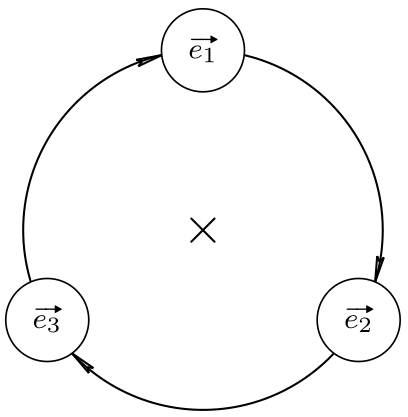
\includegraphics[width=0.5\textwidth]{vektorski_proizvod_krug.png}
        \caption*{Vektorski proizvod baznih vektora\cite{book::first}}
        \label{pic::vektorski_krug}
    \end{minipage}
\end{figure}

\par

\textbf{Formula za vektorski proizvod u ON+ bazi:} Neka su $\vek{v},\vek{u}\in
    \mathbb{V}$ i važe jednakosti
$\vek{v}=x_1\vek{e_1}+x_2\vek{e_2}+x_3\vek{e_3}$, $\vek{u}=
    y_1\vek{e_1}+y_2\vek{e_2}+y_3\vek{e_3}$. Tada:
\begin{align*}
    \vek{v}\times\vek{u} & = (x_1\vek{e_1}+x_2\vek{e_2}+x_3\vek{e_3})
    \times(y_1\vek{e_1}+y_2\vek{e_2}+y_3\vek{e_3})                        \\
                         & =x_1y_1(\vek{e_1}\times\vek{e_1})+x_1y_2
    (\vek{e_1}\times\vek{e_2})+x_1y_3(\vek{e_1}\times\vek{e_3})           \\
                         & +x_2y_1(\vek{e_2}\times\vek{e_1})+x_2y_2
    (\vek{e_2}\times\vek{e_2})+x_2y_3(\vek{e_2}\times\vek{e_3})           \\
                         & +x_3y_1(\vek{e_3}\times\vek{e_1})+x_3y_2
    (\vek{e_3}\times\vek{e_2})+x_3y_3(\vek{e_3}\times\vek{e_3})           \\
                         & =x_1y_1\vek{0}+x_1y_2\vek{e_3}-x_1y_3\vek{e_2} \\
                         & -x_2y_1\vek{e_3}+x_2y_2\vek{0}+x_2y_3\vek{e_1} \\
                         & +x_3y_1\vek{e_2}-x_3y_2\vek{e_1}+x_3y_3\vek{0} \\
                         & = \begin{vmatrix}
                                 \vek{e_1} & \vek{e_2} & \vek{e_3} \\
                                 x_1       & x_2       & x_3       \\
                                 y_1       & y_2       & y_3
                             \end{vmatrix}
\end{align*}
\par

\textbf{Matrica vektorskog množenja:} Vektorsko množenje vektora prostora
fiksiranim vektorom $\vek{v}$ je linearno preslikavanje.
Matrica $\vek{v}_\times$ tog množenja dobija se izračunavanjem
$\vek{v}\times\vek{e_1}$ (prva kolona), $\vek{v}\times\vek{e_2}$
(druga kolona), $\vek{v}\times\vek{e_3}$ (treća kolona). Na primer,
neka je $\vek{v}=x_1\vek{e_1}+x_2\vek{e_2}+x_3\vek{e_3}$.\\
Tada  $\vek{v}_\times=
    \begin{bmatrix}
        0    & x_3  & -x_2 \\
        -x_3 & 0    & x_1  \\
        x_2  & -x_1 & 0
    \end{bmatrix}$.
\par
\textbf{Površina trougla $ABC$:}
$$P_{ABC}=\frac{1}{2}ah_a=\frac{1}{2} |\vek{BC}||\vek{BA}|
    \sin(\angle{\vek{BA}\vek{BC}})=\frac{1}{2} |\vek{BC}\times\vek{BC}|$$
\par

\textbf{Orijentacija trougla $ABC$:} Trougao $ABC$ u reperu $Oe$ je zadat sa
$[A]_{Oe}=(x_1,x_2)^T$, $[B]_{Oe}=(y_1,y_2)^T$ i $[C]_{Oe}=(z_1,z_2)^T$.
Njegove koordinate možemo da proširimo sa
$[A]_{Oe}=(x_1,x_2,0)^T$, $[B]_{Oe}=(y_1,y_2,0)^T$ i $[C]_{Oe}=(z_1,z_2,0)^T$.
Kažemo da je trougao $ABC$ pozitivno orijentisan ako je
$\vek{AB}\times\vek{AC}$ istog smera kao $\vek{e_3}$,
tačnije, ako je $(y_1-x_1)(z_2-x_2)-(y_2-x_2)(z_1-x_1)>0$.
\par

\textbf{Kolinearnost tačaka:} Tri tačke su kolinearne ako je ,,površina
trougla`` koji obrazuju $0$. Dakle
$\displaystyle\frac{1}{2}\cdot|\vek{AB}\times\vek{AC}|=0$.
\par

\textbf{Da li tačka pripada trouglu:} Tačka $P$ pripada trouglu $ABC$ ako su
trouglovi $ABP$, $BCP$ i $CAP$ iste orijentacije.

\subsection{Mešoviti proizvod}
\textit{Definicija, osobine, formula za mešoviti proizvod u ON+ bazi \ocena{(dokaz)},
    zapremina paralelopipeda - T1.7 \ocena{(dokaz)}, zapremina tetraedra, orijentacija
    baze prostora, nezavisnost tri vektora prostora, primeri.}
\par
\vspace*{1cm}

\textbf{Definicija mešovitog proizvoda:} $[\vek{u},\vek{v},\vek{w}]=
    (\vek{u}\times\vek{v})\cdot\vek{w}$.
\par

\textbf{Osobine:}
\begin{enumerate}[label=\textbf{(\arabic*)}]
    \item $[\vek{u},\vek{v},\vek{w}]=-[\vek{v},\vek{u},\vek{w}]$\hspace*{1cm}
          (antisimetričnost)
    \item $[\vek{u},\vek{v},\vek{w}]=[\vek{v},\vek{w},\vek{u}]$\hspace*{1cm}
          (cikličnost)
    \item $[\alpha\cdot\vek{u}+\beta\cdot\vek{v},\vek{w},\vek{z}]=\alpha\cdot
              [\vek{u},\vek{w},\vek{z}]+\beta\cdot[\vek{v},\vek{w},\vek{z}]$
          \hspace*{1cm}(linearnost)
\end{enumerate}
\par

\textbf{Formula za mešoviti proizvod u ON+ bazi:}
$$[\vek{u},\vek{v},\vek{w}]=(\vek{u}\times\vek{v})\cdot\vek{w}= \begin{vmatrix}
        \vek{e_1} & \vek{e_2} & \vek{e_3} \\
        u_x       & u_y       & u_z       \\
        v_x       & v_y       & v_z
    \end{vmatrix}\cdot\vek{w}=\text{*sredi se*}= \begin{vmatrix}
        u_x & u_y & u_z \\
        v_x & v_y & v_z \\
        w_x & w_y & w_z
    \end{vmatrix}$$
\par

\textbf{T1.7:} Zapremina paralelopipeda jednaka je apsolutnoj vrednosti
mešovitog proizvoda tri vektora koji razapinju taj paralelopiped.
\par
\textbf{Dokaz:} Neka je dat paralelopiped $ABCDA_1B_1C_1D_1$ i neka su
$\vek{AB}=\vek{u}$, $\vek{AD}=\vek{v}$ i $\vek{AA_1}=\vek{w}$. Tada je
zapremina paralelopipeda:
\begin{align*}
    V & =P_{ABCD}h=|\vek{u}\times\vek{v}|h=\left|\left|\vek{u}\times\vek{v}\right|
    \left|\vek{w}\right|\cos(\angle{(\vek{u}\times\vek{v})\vek{w}})\right|         \\
      & =|(\vek{u}\times\vek{v}) \cdot \vek{w}|=
    |[\vek{u},\vek{v},\vek{w}]|
\end{align*}
\par

\textbf{Zapremina tetraedra:} $\frac{1}{6}|[\vek{u},\vek{v},\vek{w}]|$.
\par
\textbf{Dokaz:} Tražimo zapreminu tetraedra $ABDA_1$. Dopunimo tetraedar do
paralelopipeda $ABCDA_1B_1C_1D_1$. On je izgrađen od dve trostrane prizme
$ABDA_1B_1D_1$ i $BCDB_1C_1D_1$ koje su jednakih jednakih zapremina.
Posmatrajmo trostranu prizmu $ABDA_1B_1D_1$. Iz nje možemo da izdvojimo
tetraedre $ABDA_1$, $BDA_1B_1$ i $DA_1B_1D_1$. Tetraedri $ABDA_1$ i $BDA_1B_1$
imaju iste površine baza $ABA_1$ i $BA_1B_1$ i iste visine iz tačke $D$ pa su
im i zapremine iste. Tetraedri $ABDA_1$ i $DA_1B_1D_1$ imaju iste površine baza
$AA_1D$ i $DA_1D_1$ i iste visine iz tačke $B$ pa su im i zapremine iste.
Dakle, trostrana prizma $ADCA_1B_1D_1$ se sastoji od tri tetraedra jednakih
zapremina. Zapremina tetraedra $ABDA_1$ je jedna šestina zapremine
paralelopipeda, što se i tražilo.
\par

\textbf{Orijentacija baze prostora:} Ako je $[\vek{e_1},\vek{e_2},\vek{e_3}]>0$
onda je orijentacija pozitivna.
\par

\textbf{Nezavisnost tri vektora prostora:} Tri vektora su nezavisna ako je
zapremina paralelopipeda koji obrazuju veća od nule.

\subsection{Težište, centar mase i baricentričke koordinate}
\textit{Zakon poluge, rešavanje zakona poluge centrom mase dve tačke, centar
    mase tri tačke, ”rešavanje trougla” centrom mase tri tačke, centar mase $n$
    tačaka, težište $n$ tačaka, \ocena{dokaz da definicija težišta trougla ne zavisi
        od tačke $O$ - vežbe}, primeri, baricentričke koordinate.}
\par
\vspace*{1cm}

\textbf{Zakon poluge:} Iz jednakosti momenta sila se dobija
$|AT|:|TB|=m_B:m_A$ ili vektorski $m_A\vek{TA}+m_B\vek{TB}=\vek{0}$.
\par

\textbf{Centar mase tačaka $A(m_A)$ i $B(m_B)$:}
$\vek{OT}=\frac{1}{m_A+m_B}(m_A\vek{OA}+m_B\vek{OB})$.
\par

\textbf{Centar mase tri tačke:} $\vek{OT}=\frac{1}{m_A+m_B+m_C}
    (m_A\vek{OA}+m_B\vek{OB}+m_C\vek{OC})$.
\par

\textbf{Centar mase $n$ tačaka:} $\frac{1}{m_{A_1}+\dotsc+m_{A_n}}
    (m_{A_1}\vek{OA_1}+\dotsc+m_{A_n}\vek{OA_n})=\vek{OT}$.
\par

\textbf{Težište $n$ tačaka:} Težište $n$ tačaka se dobija kada su sve mase
jednake. Neka važi $m_{A_1}=\dotsc=m_{A_n}=m$. Tada je:
\begin{align*}
    \vek{OT} & =\frac{1}{m_{A_1}+\dotsc+m_{A_n}}(m_{A_1}\vek{OA_1}+
    \dotsc+m_{A_n}\vek{OA_n})                                       \\
             & =\frac{1}{nm}(m\vek{OA_1}+\dotsc+m\vek{OA_n})        \\
             & =\frac{1}{n}(\vek{OA_1}+\dotsc+\vek{OA_n})
\end{align*}
\par

\textbf{Dokaz da definicija težišta trougla ne zavisi od tačke $O$:} Neka su
date tačke $A$, $B$, $C$ i njihove mase i neka važi $m_{A}+m_{B}+m_{C}=M$.
Tada:
\begin{align*}
    \vek{OT}          & =\frac{1}{M}(m_{A}\vek{OA}+m_{B}\vek{OB}
    +m_{C}\vek{OC})                                              \\
    \vek{OS}+\vek{ST} & =\frac{1}{M}(m_{A}(\vek{OS}+\vek{SA})
    +m_{B}(\vek{OS}+\vek{SB})+m_{C}(\vek{OS}+\vek{SC}))          \\
    \vek{OS}+\vek{ST} & =\frac{1}{M}(m_{A}\vek{SA}+m_{B}\vek{SB}
    +m_{C}\vek{SC})+\vek{OS}                                     \\
    \vek{ST}          & =\frac{1}{M}(m_{A}\vek{SA}+m_{B}\vek{SB}
    +m_{C}\vek{SC})
\end{align*}
Za $m_{A}=m_{B}=m_{C}$ dobijamo definiciju težišta.
\par

\textbf{Baricentričke koordinate:} Baricentričke koordinate tačke $M$ su mase
koje je potrebno dodeliti tačkama $A_1,\dotsc,A_n$ tako da tačka $M$ postane
njihov centar mase. Baricentričke koordinate mogu biti homogene i nehomogene.
U slučaju $n$ tačaka $A_1(m_{A_1}),\dotsc,A_n(m_{A_n})$, homogene
baricentričke koordinate će biti $(m_{A_1}:\dotsc:m_{A_n})$. Homogene
baricentričke koordinate su određene do na proporcionalnost. Za normalizovane
ili nehomogene baricentričke koordinate važi da je $m_{A_1}+\dotsc+m_{A_n}=1$.
Za proizvoljne mase $m_{A_1},\dotsc,m_{A_n}$ nehomogene baricentričke
koordinate dobijamo sa: $(\frac{m(A_1)}{m(A_1)+\dotsc+m(A_n)},\dotsc,
    \frac{m(A_n)}{m(A_1)+\dotsc+m(A_n)})$.

\subsection{Transformacije koordinata vektora i tačaka}
\textit{Matrica prelaska, veza koordinata vektora u različitim bazama,
    primer, transformacija koordinata tačaka - formule (1.23, 1.24)
    \ocena{izvođenje}, primer.}
\par
\vspace*{1cm}

\textbf{Matrica prelaska:} Matrica u kojoj se u $i$-toj koloni nalaze
koordinate $i$-tog vektora nove baze u staroj bazi.
\par

\textbf{Transformacije koordinata tačaka:} Pretpostavimo da iz repera $Oe$
prelazimo u reper $Qf$. Dodatno, neka je $C$ matrica prelaska iz baze $e$ u
bazu $f$. Tada:
$$[X]_{Qf}=[\vek{QX}]_f=[\vek{QO}]_f+[\vek{OX}]_e=[O]_{Qf}+C[\vek{OX}]_e
    =[O]_{Qf}+C[X]_{Oe}\hspace*{0.1cm}\text{(1.23)}$$
Ako je $[X]_{Oe}=x'$, $[X]_{Qf}=x$ i $[O]_{Qf}=q$, tada dobijamo $x=q+Cx'$
(1.24).

\subsection{Transformacije koordinata u ON bazama ravni}
\label{subsec:pitanje_9}
\textit{Slučaj baza iste orijentacije, matrica rotacije, osobine matrice
    rotacije, slučaj baza različite orijentacije, matrica refleksije,
    osobine matrica refleksije, grupe $SO(2)$ i $O(2)$.}
\par
\vspace*{1cm}

\textbf{Slučaj baza iste orijentacije:} Neka su dati ON reperi ravni $Oe$ i
$Qf$ koji su iste orijentacije. Želimo da pređemo iz $Oe$ u $Qf$. Označimo sa
$\phi$ ugao $\angle{\vek{e_1}\vek{f_1}}$. Tada važe jednakosti
$\vek{f_1}=\cos(\phi)\vek{e_1}+\sin(\phi)\vek{e_2}$ i
$\vek{f_2}=-\sin(\phi)\vek{e_1}+\cos(\phi)\vek{e_2}$. Dakle
$[\vek{f_1}]_e=(\cos(\phi),\sin(\phi))^T$ i $[\vek{f_2}]_e
    =(-\sin(\phi),\cos(\phi))^T$. Odavde dobijamo formulu za ON repere iste
orijentacije: $x=q+\begin{bmatrix}
        \cos(\phi) & -\sin(\phi) \\
        \sin(\phi) & \cos(\phi)
    \end{bmatrix} x'$.
\par

\textbf{Matrica rotacije:} $R_\phi=\begin{bmatrix}
        \cos(\phi) & -\sin(\phi) \\
        \sin(\phi) & \cos(\phi)
    \end{bmatrix}$ je matrica rotacije vektora za ugao $\phi$. Rotira se u
pozitivnom smeru.
\par

\textbf{Osobine matrica rotacije:}
\begin{enumerate}[label=\textbf{(\arabic*)}]
    \item $(R_\phi)^{-1}=R_{-\phi}=(R_\phi)^T$
    \item $det(R_\phi)=1$
    \item $R_\phi R_\psi=R_{\phi+\psi}=R_\psi R_\phi$
\end{enumerate}
\par

\textbf{Slučaj baza različite orijentacije:} Neka su dati ON reperi ravni $Oe$
i $Qf$ koji su različite orijentacije. Želimo da pređemo iz $Oe$ u $Qf$.
Označimo sa $\phi$ ugao $\angle{\vek{e_1}\vek{f_1}}$. Tada važe jednakosti
$\vek{f_1}=\cos(\phi)\vek{e_1}+\sin(\phi)\vek{e_2}$ i
$\vek{f_2}=\sin(\phi)\vek{e_1}-\cos(\phi)\vek{e_2}$. Dakle
$[\vek{f_1}]_e=(\cos(\phi),\sin(\phi))^T$ i
$[\vek{f_2}]_e=(\sin(\phi),-\cos(\phi))^T$.
Odavde dobijamo formulu za ON repere različite orijentacije:
$x=q+\begin{bmatrix}
        \cos(\phi) & \sin(\phi)  \\
        \sin(\phi) & -\cos(\phi)
    \end{bmatrix} x'$.
\par

\textbf{Matrica refleksije:} $S_\phi=\begin{bmatrix}
        \cos(\phi) & \sin(\phi)  \\
        \sin(\phi) & -\cos(\phi)
    \end{bmatrix}$ je matrica refleksije u odnosu na vektor $\vek{p}$.
Prvi vektor baze koja se transformiše gradi sa vektorom $\vek{p}$ ugao
$\frac{\phi}{2}$.
\par

\textbf{Osobine matrica refleksije:}
\begin{enumerate}[label=\textbf{(\arabic*)}]
    \item $(S_\phi)^{-1}=(S_\phi)^T$
    \item $(S_\phi)^{2}=E$
    \item $det(S_\phi)=-1$
    \item $S_\phi S_\psi=R_{\phi-\psi}$
\end{enumerate}
\par

\textbf{Grupa SO(2):} $SO(2)=\{R_\phi\mid\phi\in\mathbb{R}\}$ je specijalna
ortogonalna grupa reda 2. Broj 2 označava da se posmatra ravan.
\par

\textbf{Grupa O(2):}
$O(2)=SO(2)\cup\{S_\phi\mid\phi\in\mathbb{R}\}=\{A\in
    Gl_2(\mathbb{R})\mid A^{-1}=A^T\}$
je ortogonalna grupa reda 2. Broj 2 označava da se posmatra ravan.

\subsection{Afina preslikavanja}
\textit{Definicija, pasivna i aktivna tačka gledišta, osobine afinih
    preslikavanja (T5.2) \ocena{(dokaz)}, određenost afinog preslikavanja sa tri para
    odgovarajućih tačaka, predstavljanje afinih preslikavanja ravni $3\times3$
    matricama, translacija, rotacija (oko O i oko proizvoljne tačke),
    refleksija u odnosu na pravu, skaliranje, smicanje, primeri.}
\par
\vspace*{1cm}

\textbf{Definicija afinih preslikavanja:} Neka je
$\overline{f}: \mathbb{V}\rightarrow\mathbb{V}$ linearno preslikavanje
vektorskog prostora koji je pridružen prostoru tačaka $\mathbb{E}$. Afino
preslikavanje $f: \mathbb{E}\rightarrow\mathbb{E}$ je preslikavanje tačaka koje
je indukovano sa $\overline{f}$ u smislu da važi da je $f(M)=M'$ i $f(N)=N'$
ako i samo ako je $\overline{f}(\vek{MN})=\vek{M'N'}$ za svake dve tačke $M$ i
$N$.
\par

\textbf{Pasivna tačka gledišta:} Posmatramo istu tačku iz više repera. Tada se
njene različite koordinate odnose na koordinate u različitim reperima.
\par

\textbf{Aktivna tačka gledišta:} Posmatramo istu tačku u istom reperu pre i
posle nekog afinog preslikavanja. Tada se njene različite koordinate odnose na
koordinate pre i posle preslikavanja.

\textbf{Teorema:} Svako afino preslikavanje
$f:\mathbb{E}\rightarrow\mathbb{E}$ indukovano linearnim preslikavanjem
$\overline{f}:\mathbb{V}\rightarrow\mathbb{V}$ u fiksiranom reperu $Oe$, ima
oblik: $[f(M)]_{Oe}=[\overline{f}]_{e}[M]_{Oe}+[f(O)]_{Oe}$.
\par
\textbf{Dokaz:}
\begin{align*}
    [f(M)]_{Oe}-[f(O)]_{Oe} & =[\vek{Of(M)}]_e-[\vek{Of(O)}]_e
    =[\vek{Of(M)}]_e+[\vek{f(O)O}]_e                                         \\
                            & =[\vek{f(O)f(M)}]_e=[\overline{f}(\vek{OM})]_e
    =[\overline{f}]_e[\vek{OM}]_e                                            \\
                            & =[\overline{f}]_e[M]_{Oe}                      \\
    [f(M)]_{Oe}             & =[\overline{f}]_{e}[M]_{Oe}+[f(O)]_{Oe}
\end{align*}
\textbf{Napomena:} Kolone matrice $[\overline{f}]_e$ su zapravo slike baznih
vektora baze $e$ ($i$-ta kolona će biti $\overline{f}(\vek{e_i})$).
\par

\textbf{Osobine afinih preslikavanja ravni (T5.2):}
\begin{enumerate}[label=\textbf{(\arabic*)}]
    \item Preslikavaju prave u prave.
          \par
          \textbf{Dokaz:} S obzirom da je svako afino preslikavanje indukovano
          linearnim preslikavanjem vektorskog prostora, a linearno
          preslikavanje vektorskog prostora čuva kolinearnost, tada i afino
          preslikavanje čuva kolinearnost, odnosno, slika prave u prave.

    \item Čuvaju razmeru kolinearnih duži.
          \par
          \textbf{Dokaz:} Analogno prošloj osobini.

    \item Čuvaju paralelnost pravih.
          \par
          \textbf{Dokaz:} Ako se posmatraju po dve tačke na dve paralelne
          prave, dobijamo 2 kolinearna vektora. Odavde se analogno završava
          dokaz.

    \item Odnos površina slike i originala jednak je $|det(m_{ij})|$.
          \par
          \textbf{Dokaz:} Napomenimo da je $M=\left\{m_{ij}\right\}$ zapravo matrica
          $[\overline{f}]_e$. Zbog jednostavnijeg zapisa i jer je reper
          fiksiran ćemo izostaviti reper iz zapisa. Neka je $f(O)=O'$,
          $f(A)=A'$ i $f(B)=B'$. Površina trougla $OAB$ je
          $\frac{1}{2}|det(\vek{OA}\vek{OB})|$, a površina trougla $O'A'B'$ je
          $\frac{1}{2}|det(\vek{O'A'}\vek{O'B'})|$. Takođe su
          $\vek{O'A'}=M\vek{OA}$ i $\vek{O'B'}=M\vek{OB}$. Za kraj,
          koristimo svojstvo $det(AB)=det(A)det(B)$.
          \begin{align*}
              1           & =\frac{det(\vek{OA}\vek{OB})}{det(\vek{OA}\vek{OB})}       \\
              det(a_{ij}) & =\frac{det((M\vek{OA})(M\vek{OB}))}{det(\vek{OA}\vek{OB})} \\
              det(a_{ij}) & =\frac{det(\vek{O'A'}\vek{O'B'})}{det(\vek{OA}\vek{OB})}   \\
          \end{align*}

    \item Čuvaju centar mase i baricentričke koordinate.
          \par
          \textbf{Dokaz:} Centar mase se definiše kao linearna kombinacija
          vektora, a kako je u osnovi afinog preslikavanja linearnost, čuva
          se centar mase.

    \item Preslikavanja za koje važi $det(a_{ij})>0$ čuvaju orijentaciju,
          inače menjaju.
          \par
          \textbf{Dokaz:} Po algebarskoj definiciji, dve baze su iste
          orijentacije ako je determinanta matrice prelaska iz jedne u drugu
          veća od nule. Ovo je aktivna varijanta ove definicije.
\end{enumerate}
\par

\textbf{Određenost afinog preslikavanja sa tri para odgovarajućih tačaka:}
Neka su date tačke $O=(0,0)$, $A=(1,0)$ i $B=(0,1)$. Hoćemo da odredimo afino
preslikavanje koje slika $O$, $A$ i $B$ u proizvoljne nekolinearne tačke $O'$,
$A'$ i $B'$. Važi da je $f(O)=O'$, a kolone matrice $[\overline{f}]_{e}$ su
kolone vektora $\vek{O'A'}$ i $\vek{O'B'}$ čime smo odredili afino
preslikavanje. Hoćemo da preslikamo proizvoljne nekolinearne tačke $E$, $F$ i
$G$ u $E'$, $F'$ i $G'$. Postoji afino preslikavanje $g$ koje slika tačke $O$,
$A$ i $B$ u $E$, $F$ i $G$ i postoji afino preslikavanje $h$ koje slika tačke
$O$, $A$ i $B$ u $E'$, $F'$ i $G'$. Traženo preslikavanje će biti
$h\circ g^{-1}$ (potrebno je znati i na primeru).
\par

\textbf{Translacija:}
$\mathcal{T}_{\vek{t}}=\begin{bmatrix}
        1 & 0 & x_t \\
        0 & 1 & y_t \\
        0 & 0 & 1
    \end{bmatrix}$, gde je $\vek{t}=(x_t,y_t)$ vektor za koji se translira.
\par

\textbf{Rotacija oko $O$:}
$\mathcal{R}_\phi=\begin{bmatrix}
        \cos(\phi) & -\sin(\phi) & 0 \\
        \sin(\phi) & \cos(\phi)  & 0 \\
        0          & 0           & 1
    \end{bmatrix}$, gde je $\phi$ ugao za koji se rotira.
\par

\textbf{Rotacija oko proizvoljne tačke:}
$\mathcal{T}_{\vek{OM}}\circ\mathcal{R}_\phi\circ\mathcal{T}_{\vek{MO}}$, gde
je $M$ tačka oko koje rotiramo, a $\phi$ ugao za koji rotiramo.
\par

\textbf{Refleksija u odnosu na pravu koja prolazi kroz $O$:}
$\mathcal{S}_{p_0}=\begin{bmatrix}
        cos(\phi) & sin(\phi)  & 0 \\
        sin(\phi) & -cos(\phi) & 0 \\
        0         & 0          & 1
    \end{bmatrix}$, gde je $\frac{\phi}{2}$ ugao između $x$ ose i $p_0$.
Refleksija u odnosu na pravu koja prolazi kroz proizvoljnu tačku se dobija
analogno kao rotacija.
\par

\textbf{Skaliranja sa centrom u tački $O$}:
$\mathcal{H}_{\lambda_1,\lambda_2}=\begin{bmatrix}
        \lambda_1 & 0         & 0 \\
        0         & \lambda_2 & 0 \\
        0         & 0         & 1
    \end{bmatrix}$, gde je $\lambda_1$ koeficijent skaliranja u pravcu
prvog baznog vektora, a $\lambda_2$ koeficijent skaliranja u pravcu
drugog baznog vektora. Skaliranje sa centrom u proizvoljnoj tački analogno
rotaciji.
\par

\textbf{Smicanje:} Smicanje preslikava kvadrat u pravougaonik iste površine.
Matrice smicanja:
\begin{enumerate}[label=]
    \item $\mathcal{S}_x(\lambda)=\begin{bmatrix}
                  x & \lambda & 0 \\
                  0 & y       & 0 \\
                  0 & 0       & 1
              \end{bmatrix}$, gde je $\lambda$ koeficijent smicanja u pravcu $x$ ose.
    \item $\mathcal{S}_y(\lambda)=\begin{bmatrix}
                  x       & 0 & 0 \\
                  \lambda & y & 0 \\
                  0       & 0 & 1
              \end{bmatrix}$, gde je $\lambda$ koeficijent smicanja u pravcu $y$ ose.
\end{enumerate}

\subsection{Izometrije ravni i prostora}
\textit{Defincija, direktne i indirekne izometrije, ortogonalne matrice i
    njihova determinanta, opis afinih transformacija ravni (pitanje 9), rotacija
    oko prave u prostoru, rotacije oko koordinatnih osa, Rodrigezova formula,
    refleksija u odnosu na ravan (računanje), Prva Ojlerova teorema, Ojlerovi
    uglovi, Druga Ojlerova teorema, \ocena{veza sopstvenih i svetskih rotacija - smisao,
        slučaj zaključanog žiroskopa}.}
\par
\vspace*{1cm}

\textbf{Definicija izometrije:} Preslikavanje koje čuva dužine u euklidskom prostoru
$\mathbb{E}$ proizvoljne dimenzije.
\par

\textbf{Direktne izometrije:} Čuvaju orijentaciju (kretanja).
\par

\textbf{Indirektne izometrije:} Menjaju orijentaciju.
\par

\textbf{Ortogonalna matrica i njena determinanta:} Matrica $A$ za koju važi
$AA^T=E$. Za determinantu ortogonalne matrice važi
$1=det(E)=det(AA^T)=det(A)det(A^T)=det(A)det(A)=det(A)^2$. Odatle važi da je
$\pm 1=det(A)$.
\par

\textbf{Opis afinih transformacija ravni:} \hyperref[subsec:pitanje_9]{Pitanje 9}.
\par

\textbf{Matrica rotacije oko $x$ ose:} $R_x(\phi)=\begin{bmatrix}
        1 & 0          & 0           \\
        0 & \cos(\phi) & -\sin{\phi} \\
        0 & \sin(\phi) & \cos(\phi)
    \end{bmatrix}$
\par
\textbf{Matrica rotacije oko $y$ ose:} $R_y(\phi)=\begin{bmatrix}
        \cos(\phi)  & 0 & \sin{\phi} \\
        0           & 1 & 0          \\
        -\sin(\phi) & 0 & \cos(\phi)
    \end{bmatrix}$
\par
\textbf{Matrica rotacije oko $z$ ose:} $R_z(\phi)=\begin{bmatrix}
        \cos(\phi) & -\sin{\phi} & 0 \\
        \sin(\phi) & \cos(\phi)  & 0 \\
        0          & 0           & 1
    \end{bmatrix}$
\par
\textbf{Rotacija oko proizvoljne prave koja sadrži $O$ (Rodrigezova formula):}
Neka je dat ON reper $Oe$ i neka su date tačka $M$ i prava $p_0$ koja sadrži
tačku $O$ i ugao $\phi$ za koji rotiramo tačku $M$ oko prave
$p_0$. Neka je jedinični vektor pravca prave $p_0$ vektor $\vek{p}$. Posmatrajmo
ravan $\alpha$ koja sadrži tačku $M$ i njen normalni vektor je vektor
$\vek{p}$. Neka je $\alpha\cap p_0 =\{O'\}$ i neka su $\vek{x}=\vek{OM}$,
$\vek{x_1}=\vek{OO'}$ i $\vek{x_2}=\vek{O'M}$. Tada:
\begin{align*}
    \vek{x}             & =\vek{x_1}+\vek{x_2} = \lambda\vek{p}+\vek{x_2}                                  \\
    \vek{p}\cdot\vek{x} & =\lambda(\vek{p}\cdot\vek{p})+\vek{p}\cdot\vek{x_2} =\lambda|\vek{p}|^2 =\lambda
\end{align*}
Tada za $x_1$ dobijamo $x_1=p\lambda=p(p^Tx)=(pp^T)x$, a za $x_2$ dobijamo
$x_2=x-x_1=Ex-(pp^T)x=(E-pp^T)x$. Neka je sada $M'$ tačka koja se dobija
rotacijom tačke $M$ oko prave $p$ za ugao $\phi$. Možemo da posmatramo
ortogonalnu bazu $(\vek{p},\vek{x_2},\vek{p}\times\vek{x_2})$. Tada je:
\begin{align*}
    \vek{O'M'} & =\cos(\phi)\vek{x_2}+\sin(\phi)(\vek{p}\times\vek{x_2})             \\
               & =\cos(\phi)\vek{x_2}+\sin(\phi)(\vek{p}\times(\vek{x_1}+\vek{x_2})) \\
               & =\cos(\phi)\vek{x_2}+\sin(\phi)(\vek{p}\times\vek{x})
\end{align*}
Na kraju dobijamo koordinate tačke $M'$:
$$[M']_{Oe}=[\vek{OM'}]_e=[\vek{OO'}]_e+[\vek{O'M'}]_e=(pp^T)x+\cos(\phi)(E-pp^T)x+\sin(\phi)\vek{p}_\times x$$
Možemo da izdvojimo matricu
$[R_p(\phi)]_e=pp^T+\cos(\phi)(E-pp^T)+\sin(\phi)\vek{p}_\times$
koju nazivamo Rodrigezova formula.
\par

\textbf{Refleksija u odnosu na ravan koja sadrži O:}
\label{refleksija_u_odnosu_na_ravan} Neka je dat ON reper $Oe$,
ravan $\alpha$ koja prolazi kroz $O$ zadata jediničnim normalnim vektorom
$\vek{p}$ i neka je data tačka $M$ na koju hoćemo da primenimo refleksiju u
odnosu na ravan i neka se tom refleksijom dobija tačka $M'$. Neka je
$\alpha\cap MM'=\{O'\}$. Dobijamo
$\vek{OM'}=\vek{OM}+\vek{MM'}=\vek{OM}-2\vek{O'M}$. Neka su sa $p$ i $x$
označene koordinate vektora $\vek{p}$ i $\vek{OM}$.

Analogno sa pitanjem za Rodrigezovu formulu:
\begin{align*}
    \vek{O'M}             & =\lambda\vek{p}                                                \\
    \vek{p}\cdot\vek{O'M} & =\vek{p}\cdot(\vek{O'O}+\vek{OM})=\vek{p}\cdot\vek{OM}=\lambda
\end{align*}
Odavde, u koordinatama dobijamo $[\vek{O'M}]_e=(pp^T)x$. Na kraju dobijamo
koordinate preslikane tačke:
$$[\vek{OM'}]_e=Ex-2(pp^T)x$$
Možemo da izdvojimo matricu: $[S_\alpha]_e=E-2pp^T$ koju nazivamo matrica
refleksije u odnosu na ravan.
\par

\textbf{Prva Ojlerova teorema:} Svako kretanje koje ima fiksiranu tačku
$O'$ se može predstaviti kao rotacija oko neke orijentisane
prave koja sadrži tačku $O'$.
\par

\textbf{Druga Ojlerova teorema:} Svako kretanje koje fiksira $O$ se može
izraziti kao kompozicija tri sopstvene rotacije oko koordinatnih osa:
$\mathcal{R}_{Ox_2}(\phi)\circ \mathcal{R}_{Oy_1}(\theta)\circ \mathcal{R}_{Oz}(\psi)$ gde su uglovi
$\phi,\psi\in[0,2\pi)$, $\theta\in[-\frac{\pi}{2},\frac{\pi}{2}]$. Uglovi $\phi$,
$\theta$, $\psi$ se nazivaju Ojlerovi uglovi. Prvom rotacijom se $Oxyz$ slika u
$Ox_1y_1z_1$, drugom rotacijom u $Ox_2y_2z_2$ i trećom rotacijom u $Ox_3y_3z_3$.
\par

\textbf{Veza sopstvenih i svetskih koordinata:}
$[\mathcal{R}_{Ox_2}(\phi)\circ \mathcal{R}_{Oy_1}(\theta)\circ \mathcal{R}_{Oz}(\psi)]_e=[R_{Oz}]_e(\psi)\cdot [R_{Oy}]_e(\theta)\cdot [R_{Ox}](\phi)$.
\par

\textbf{Slučaj zaključanog žiroskopa:} Javlja se kada se ravni
$Oxy$ i $Oy_3z_3$ poklope. Tada je $|Oz|=|Ox_3|$ zbog čega imamo jedan stepen slobode manje.

\subsection{Kvaternioni}
\textit{Definicija, sabiranje, množenje, osobine, inverzni
    kvaternion, primeri, \ocena{konjugacija kvaternionom i izometrije}.}
\par
\vspace*{1cm}

\textbf{Definicija kvaterniona:}
$\mathbb{H}=\{xi+yj+zk+w\mid x,y,z,w\in\mathbb{R}\}$, gde su $i$, $j$ i $k$
imaginarne jedinice.
\par

\textbf{Sabiranje kvaterniona:} Normalno.
\par

\textbf{Množenje kvaterniona:} $i j=k=-j i$ i $i^2=j^2=k^2=-1$.
\par

\textbf{Realni i imaginarni deo:} Realni deo: $\mathcal{R}(q)=w$, imaginarni
deo: $\mathcal{I}(q)=x i +y j +z k=\vek{v}$. Važi
$q=xi+yj+zk+w=\mathcal{I}(q)+\mathcal{R}(q)=[(x,y,z),w]=[\vek{v},w]$.
\par

\textbf{Osobine:}
\begin{enumerate}[label=\textbf{(\arabic*)}]
    \item $q+q_1=[\vek{v},w]+[\vek{v_1},w_1]=[\vek{v}+\vek{v_1},w+w_1]$
    \item $q q_1=[\vek{v},0][\vek{v_1},0]=[\vek{v}\times\vek{v_1},-\langle\vek{v},\vek{v_1}\rangle]$
    \item $q q_1=[\vek{v},w_1][\vek{v_1},w_1]=[\vek{v}\times\vek{v_1}+w \vek{v_1}+w_1\vek{v},w w_1-\langle\vek{v},\vek{v_1}\rangle]$\\
          Napomena: $\langle\vek{v},\vek{u}\rangle$ je drugi zapis za skalarni proizvod.
\end{enumerate}

\textbf{Konjugovani kvaternion:} $\overline{q}=-x i -y j -z k+w$.
\par

\textbf{Inverzni kvaternion:} $q q^{-1}=1$. Osobina:
$q \overline{q}=|q|^2 \implies q^{-1}=\frac{\overline{q}}{|q|^2}$.
\par

\textbf{Konjugacije kvaternionom:} Svaki kvaternion različit od nule određuje
konjugaciju $C_q=qpq^{-1}$. Dve konjugacije su iste ako i samo ako važi
$q=\lambda h$, gde je $\lambda\in\mathbb{R}$. \par
\textbf{Izometrije:} Ako je $q=[\vek{v}\sin(\frac{\alpha}{2}),\cos(\frac{\alpha}{2})]$
tada konjugacija $C_q$ u prostoru imaginarnih kvaterniona indukuje rotaciju oko jediničnog
vektora $\vek{v}$ za ugao $\alpha$ u pozitivnom smeru.
\par

\subsection{Afina geometrija ravni}
\textit{Predstavljanje prave, razne jednačine pravih, normalni vektor prave,
    vektor pravca prave, presek dve prave zadate jednačinama, presek pravih
    zadatih tačkom i vektorom pravca \ocena{(dokaz)}, presek dve duži, parametarsko
    zadavanje trougla, paralelograma.}
\par
\vspace*{1cm}

\textbf{Implicitna jednačina prave:} $ax+by+c=0$.
\par

\textbf{Parametarska jednačina prave:} $M(t)=P+t\vek{p}$.
\par

\textbf{Normalni vektor:} Iz implicitnog zapisa možemo da pročitamo normalni
vektor $\vek{n_p}=(a,b)^T$.
\par

\textbf{Vektor pravca:} Iz parametarskog zapisa možemo da pročitamo vektor
pravca $\vek{p}$.
\par

\textbf{Presek pravih:} Dobija se rešavanjem dve jednačine prave sa dve
nepoznate.
\par

\textbf{Presek dve duži:} Duž $AB$ možemo da zadamo parametarski sa
$M(t)=A+t\vek{AB}$, $t\in[0,1]$. Slično, duž $CD$ možemo da zadamo parametarski sa $N(s)=C+s\vek{CD}$, $s\in[0,1]$.
Za presek dve duži određujemo tačku preseka kao za prave, a zatim određujemo da li važi da su
parametri $t$ i $s$ za tačku preseka iz intervala $[0,1]$.
\par

\textbf{Parametarsko zadavanje trougla i paralelograma:} Trougao možemo da
zadamo sa $M(t_1,t_2)=A+t_1\vek{AB}+t_2\vek{AC}$, $t_1,t_2\in[0,1]$, $t_1+t_2\leq1$.
Paralelogram možemo da zadamo sa $M(t_1,t_2)=A+t_1\vek{AB}+t_2\vek{AC}$, $t_1,t_2\in[0,1]$.

\subsection{Ravan u prostoru}
\textit{Zadavanje ravni tačkom i normalnim vektorom \ocena{(dokaz)}, skiciranje ravni,
    specijalni slučajevi ravni, parametarska jednačina ravni, jednačina ravni kroz
    3 tačke, primeri.}
\par
\vspace*{1cm}

\textbf{Zadavanje ravni tačkom i normalnim vektorom:} Neka je dat normalni
vektor $\vek{n_\alpha}=(a,b,c)^T$ i tačka $P=(x_1,y_1,z_1)$ koja pripada ravni.
Posmatrajmo tačku sa ravni $A=(x,y,z)$. Važi da je
$\vek{PA}\cdot\vek{n_\alpha}=0$. Odavde:
$\vek{PA}\cdot\vek{n_\alpha}=(x-x_1,y-y_1,z-z_1)\cdot(a,b,c)=ax+by+cz-
    (ax_1+by_1+cz_1)=0$. Ako obeležimo $d=-(ax_1+by_1+cz_1)$ dobijamo
$ax+by+cz+d=0$.
\par

\textbf{Skiciranje ravni:} Skiciranje ravni može da se vrši tako što se prvo
izračunaju i označe preseci sa osama. U slučaju da ima tačno jedan presek,
ravan će prolaziti kroz tačke preseka i biće paralelna sa osama koje ne
seče. U slučaju da ima tačno dva preseka, ravan će prolaziti kroz tačke
preseka i biće paralelna sa osom koju ne seče. U slučaju da ima tačno tri
preseka, imamo tri tačke koje određuju ravan, pa možemo da je skiciramo.
\par

\textbf{Parametarska jednačina ravni:} $M(t,s)=A+t\vek{v}+s\vek{u}$, gde je $t,s\in\mathbb{R}$, $A$
tačka koja pripada ravni, a $\vek{v}$ i $\vek{u}$ su nekolinearni vektori
paralelni sa ravni.
\par

\textbf{Jednačina ravni kroz tri tačke:} Ako su date nekolinearne tačke $A$,
$B$ i $C$, tada je jednačine ravni: $M(t,s)=A+t\vek{AB}+s\vek{AC}$.
Ako su tačke kolinearna ne može se jednoznačno odrediti ravan koja ih sadrži.
\par

\subsection{Prava u prostoru}
\textit{Parametarska i ”kanonska” jednačina prave, prava AB i podela duži AB
    na jednake delove, prava kao presek dve ravni, pramen ravni, primeri.}
\par
\vspace*{1cm}

\textbf{Parametarska jednačina:} $M(t)=A+t\vek{p}$, gde je $A$ tačka na pravoj,
a $\vek{p}$ je vektor pravca.
\par

\textbf{,,Kanonska`` jednačina:} ,,Kanonska`` je pod navodnicima jer bi nešto
što je kanonsko trebalo da bude jedinstveno, što ova jednačina ne mora da bude.
Kanonska jednačina prave:
$\frac{x-x_0}{p_x}=\frac{y-y_0}{p_y}=\frac{z-z_0}{p_z}=t$. Dopuštamo da $p_x$,
$p_y$ ili $p_z$ budu nula.
\par

\textbf{Prava $AB$:} Ako su date dve različite tačke $A$ i $B$ možemo
jednoznačno da odredimo pravu koja prolazi kroz njih formulom
$M(t)=A+t\vek{AB}$.
\par

\textbf{Podela duži $AB$ na jednake delove:} Ako želimo da podelimo duž $AB$ na
$n$ jednakih delova i želimo da nađemo $m$-tu tačku podele to radimo po formuli:
$T_m=A+\frac{m}{n}\vek{AB}$, važi da je $T_0=A$ i $T_n=B$.
\par

\textbf{Prava kao presek dve ravni:} Dobija se kao rešenje sistema dve
jednačine od tri nepoznate. Može da nema rešenja (ravni su paralelne), ima
beskonačno mnogo rešenja koja formiraju pravu (ravni se seku po pravoj) ili ima
beskonačno mnogo rešenja koja formiraju ravan (ravni se poklapaju).
\par

\textbf{Pramen ravni:} Ako se dve ravni seku po pravoj, njihovom linearnom
kombinacijom se dobija svaka ravan koja sadrži tu pravu i ovo se naziva pramen
ravni. U opštem primeru, neka je $\alpha: a_1x+b_1y+c_1z+d_1=0$ i
$\beta: a_2x+b_2y+c_2z+d_2=0$. Tada je pramen ravni:
$\lambda_1\cdot(a_1x+b_1y+c_1z+d_1)+\lambda_2(a_2x+b_2y+c_2z+d_2)=0$.

\subsection{Međusobni položaji pravih i ravni}
\label{subsec:pitanje_16}
\textit{Međusobni položaji dve prave (zadatih tačkom i vektorom pravca) u
    prostoru, međusobni položaj prave i ravni, međusobni položaji dve ravni,
    mimoilazne prave, zajednička normala - T4.3 \ocena{(dokaz)}, rastojanje mimoilaznih
    pravih - T4.4 \ocena{(dokaz)}.}
\par
\vspace*{1cm}

\textbf{Međusobni položaj dve prave:} Dve prave mogu da budu paralelne,
mimoilazne, da se poklapaju i da se seku. Možemo da rešavamo četiri jednačine sa
tri nepoznate. Ako postoji jedno rešenje onda se seku. Ako postoji beskonačno
mnogo rešenja onda se poklapaju. Ako nema rešenja, a vektori su kolinearni onda
su prave paralelne. Ako sistem nema rešenja, onda su mimoilazne.
\par

\textbf{Međusobni položaj prave i ravni:} Prava i ravan mogu da budu paralelne,
da se seku ili da ravan sadrži pravu. Ako sistem jednačina ima jedinstveno
rešenje onda se seku, ako ima beskonačno mnogo rešenja onda ravan sadrži pravu,
inače su paralelne.
\par

\textbf{Međusobni položaj dve ravni:} Dve ravni mogu da se poklapaju, budu
paralelne ili da se seku. Slučajevi su analogni slučajevima međusobnog položaja
prave i ravni.
\par

\textbf{Mimoilazne prave:} Dve prave za koje ne postoji ravan koja ih sadrži.
\par

\textbf{T4.3:} Mimoilazne prave $p$ i $q$ imaju jedinstvenu zajedničku normalu.
\par
\textbf{Dokaz:} Neka je ravan $\alpha$ paralelna pravoj $q$ i sadrži pravu $p$ i
neka je ravan $\beta$ paralelna pravoj $p$ i sadrži pravu $q$. Neka ravan $\gamma$
sadrži pravu $p$ i normalna je na ravan $\alpha$.
Neka je prava $p_1$ presek ravni $\beta$ i $\gamma$. Tada je
$p$ paralelno sa $p_1$, po konstrukciji, i $p_1$ seče $q$, inače bi
$p$ i $q$ bili paralelni, što je kontradikcija sa pretpostavkom.
Prave $p_1$ i $q$ se seku u nekoj tački $N$. Neka je prava $n$ normalna
na ravan $\beta$ i prolazi kroz tačku $N$, odakle je normalna i na pravu
$q$. Kako je prava $n$ normalna i na ravan $\alpha$ i seče pravu $p$
(jer seče i pravu $p_1$), tada su i $p$ i $n$
normalne, što smo i hteli da dokažemo.\par
Prava $n$ je jedinstvena, jer je tačka $N$ jedinstvena.
\par

\textbf{T4.4} Rastojanje između mimoilaznih pravih je:
$\frac{|[\vek{p},\vek{q},\vek{PQ}]|}{|p\times q|}$ gde su $P$ i $\vek{p}$ tačka
i vektor pravca prave $p$, a $Q$ i $\vek{q}$ tačka i vektor pravca prave $q$.
\par
\textbf{Dokaz:} U brojiocu je zapravo zapremina paralelopipeda, a u imeniocu je
površina baze zbog čega se deljenjem tačno dobija visina koju tražimo.
\par

\subsection{Projekcije}
\textit{Normalna projekcija na ravan $Oxy$ (je linearno preslikavanje),
    normalna projekcija na\\proizvoljnu ravan \ocena{(dokaz)}, centralna projekcija, \ocena{formule
        centralne projekcije iz $C(0,0,0)$ na ravan $z=f$}, kartografske projekcije,
    definicija \ocena{i formule} stereografska projekcija.}
\par
\vspace*{1cm}

\textbf{Normalna projekcija na ravan $Oxy$:} Matrica $\begin{bmatrix}
        1 & 0 & 0 & 0 \\
        0 & 1 & 0 & 0 \\
        0 & 0 & 0 & 0 \\
        0 & 0 & 0 & 1
    \end{bmatrix}$ je matrica normalne projekcije na ravan $Oxy$.
\par

\textbf{Normalna projekcija na proizvoljnu ravan:} Neka je $\alpha$ ravan koja
prolazi kroz $O$ zadata jediničnim normalnim vektorom $\vek{p}$ i neka je data
tačka $M$ koju hoćemo da projektujemo na ravan i neka se tom projekcijom dobija
tačka $M'$. Označimo kolone vektora $\vek{p}$, $\vek{OM}$ i $\vek{OM'}$ redom
sa $p$, $x$, $x'$. Tada, analogno \hyperref[refleksija_u_odnosu_na_ravan]
{dokazu formule refleksije u odnosu na ravan},
dobijamo formulu: $x'=(E-pp^T)x$.
\par

\textbf{Centralna projekcija:} Za centralnu projekciju je potrebno da fiksiramo
ravan na koju projektujemo i tačku u odnosu na koju projektujemo (iz koje
posmatramo).
\par

\textbf{Formula centralne projekcije u odnosu na tačku $C(0,0,0)$ na ravan
    $z=d$:} Posmatrajmo proizvoljnu tačku $M(x,y,z)$. Neka je njena projekcija
tačka $M'(x',y',z')$. Tada je $x'=\frac{d}{z}x$, $y'=\frac{d}{z}y$
i $z'=\frac{d}{z}z=d$. Ovo možemo izraziti matrično preko homogenih
koordinata. Neka je $x'=\frac{x_1'}{x_4'}$, $y'=\frac{x_2'}{x_4'}$ i
$z'=\frac{x_3'}{x_4'}$. Tada se centralna projekcija može predstaviti formulom:
$\begin{bmatrix}
        x_1' \\
        x_2' \\
        x_3' \\
        x_4'
    \end{bmatrix}=\begin{bmatrix}
        d & 0 & 0 & 0 \\
        0 & d & 0 & 0 \\
        0 & 0 & d & 0 \\
        0 & 0 & 1 & 0
    \end{bmatrix}\begin{bmatrix}
        x \\
        y \\
        z \\
        1
    \end{bmatrix}$.
\par

\textbf{Kartografske projekcije:} Projektuju zakrivljene površine na ravan.
\par

\textbf{Definicija stereografske projekcije:} Specijalan slučaj centralne projekcije,
vrsta kartografske projekcije kojom se jedinična sfera projektuje na ravan.
Centar projekcije je neka tačka sfere, a ravan na koju se projektuje tangira
sferu.
\par

\textbf{Izvođenje formula stereografske projekcije:} Neka je $C=(0,0,1)$ i
$z=-1$. Posmatrajmo tačku na sferi $M=(x,y,z)$ i pravu
$p(\lambda)=C+\lambda\vek{CM}$. Važi $x'=\lambda x$, $y'=\lambda y$ i
$z'=\lambda z+\lambda=-1$. Odavde dobijamo $\lambda=\frac{1}{1-z}$. Na kraju
dobijamo formule stereografske projekcije: $x'=\frac{x}{1-z}$,
$y'=\frac{y}{1-z}$ i $z'=-1$.


\subsection{Uglovi između pravih i ravni}
\textit{Merenje uglova (stepeni, radijani, nagib u procentima), ugao između 2
    prave, ugao između prave i ravni, ugao između dve ravni, \ocena{ugao između
        pljosni tetraedra (na dva načina)}, računski primeri.}
\par
\vspace*{1cm}

\textbf{Merenje uglova:} Veza stepena i radijana: $180^\circ=\pi$. Radijan
predstavlja odnos dužine luka i dužine poluprečnika.
\par

\textbf{Merenje nagiba u procentima:} Merimo ugao između hipotenuze i
nalegle katete. Označimo dužinu te katete sa $a$, a dužinu druge katete
sa $b$. Tada će nagib biti $\frac{b}{a}100\%$.
Dakle, ako je dužina jedne katete $1$ metar, a dužina druge katete $5$
centimetara, tada će nagib hipotenuze biti $5\%$.
\par

\textbf{Ugao između dve prave:} Određuje se kao ugao između vektora pravca tih
pravih.
\par

\textbf{Ugao između prave i ravni:} Određuje se kao
$\frac{\pi}{2}-\angle{\vek{n_\alpha}\vek{p}}$ gde je $\vek{n_\alpha}$ normalni
vektor ravni, a $\vek{p}$ vektor pravca prave.
\par

\textbf{Ugao između dve ravni:} Ugao između njihovih normalnih vektora.
\par

\textbf{Ugao između pljosni tetraedra:}
\begin{enumerate}[label=\textbf{(\arabic*)}]
    \item[\textbf{(1. način)}] Posmatrajmo jediničnu kocku $ABCDA'B'C'D'$. Tačke $A$, $C$, $B'$ i
          $D'$ formiraju pravilni tetraedar. Lako možemo da odredimo
          koordinate ovih tačaka, a zatim računski dobijamo da je ugao
          između pljosni $\arccos(\frac{1}{3})$.
    \item[\textbf{(2. način)}] Posmatrajmo pravilni jedinični tetraedar $ABCD$. Označimo sredinu
          stranice $AB$ sa $M$. Izdvojimo trougao $MDC$. Zanima nas ugao
          $\angle CMD$. Važi $|MD|=\frac{\sqrt{3}}{2}$, $|DC|=1$ i
          $|MC|=\frac{\sqrt{3}}{2}$. Preko kosinusne teoreme za trougao $CMD$
          kod ugla $\angle CMD$ dobijamo
          $|DC|^2=|MD|^2+|MC|^2-2|MD||MC|\cos(\angle CMD)$, odakle je
          $\angle CMD=\arccos(\frac{1}{3})$.
\end{enumerate}

\subsection{Rastojanja}
\textit{Rastojanje između tačke i prave (sa izvođenjem), rastojanje između
    tačke i ravni \ocena{(dokaz)}, rastojanje između mimoilaznih pravih (pitanje 16).}
\par
\vspace*{1cm}

\textbf{Rastojanje između tačke i prave:} Neka je data prava $p$ i tačka $A$
čije rastojanje se traži. Možemo da izaberemo neku tačku $B$ na pravoj i da
izračunamo površinu paralelograma zadatog vektorima: $\vek{AB}$ i $\vek{p}$.
Tada se tražena visina dobija formulom
$d(A,p)=\frac{|\vek{AB}\times\vek{p}|}{|\vek{p}|}$.
\par
\textbf{Rastojanje između tačke i ravni:} Potpuno analogno osim što se umesto
površine i dužine koristi zapremina i površina.
\par

\textbf{Rastojanje između mimoilaznih pravih:}
\hyperref[subsec:pitanje_16]{Pitanje 16}.

\subsection{Prodor prave kroz trougao}
\textit{Uslov da prava prodire trougao \ocena{(objašnjenje)}, određivanje prodorne
    tačke, primer. Presek trougla i ravni.}
\par
\vspace*{1cm}

\textbf{Uslov da prava prodire trougao (objašnjenje):} Neka je dat trougao
$ABC$ i prava $p$ određena tačkom $P$ i vektorom $\vek{p}$. Označimo sa
$\vek{u}$, $\vek{v}$ i $\vek{w}$ vektore $\vek{PA}$, $\vek{PB}$ i $\vek{PC}$.
Možemo da odredimo orijentaciju vektora $(\vek{u},\vek{v},\vek{p})$,
$(\vek{v},\vek{w},\vek{p})$ i $(\vek{w},\vek{u},\vek{p})$. Ako su sve iste
orijentacije, onda će presek pripadati trouglu. Orijentacije određujemo
mešovitim proizvodom. Specijalno, ako je tačno jedan od mešovitih proizvoda
jednak nula, tada će presek biti na nekoj od stranica. Ako je mešoviti proizvod
neka dva jednak nula tada će tačka preseka biti podudarna sa jednim od temena.
\par

\textbf{Određivanje prodorne tačke:} Označimo sa $M$ presek ravni koja sadrži
trougao sa pravom $p$. Tada će važiti $0=[\vek{AB},\vek{AC},\vek{AM}]$ jer su
ovi vektori komplanarni i neka je $\vek{AB}=\vek{v}-\vek{u}$,
$\vek{AC}=\vek{w}-\vek{u}$ i $\vek{AM}=t\vek{p}-\vek{u}$. Iz jednakosti
dobijamo:
\begin{align*}
    0                         & = [\vek{v}-\vek{u},\vek{w}-\vek{u},t\vek{p}-\vek{u}]                              \\
                              & = [\vek{v},-\vek{u},-\vek{u}]+[\vek{v},-\vek{u},t\vek{p}]+
    [\vek{v},\vek{w},-\vek{u}]+[\vek{v},\vek{w},t\vek{p}]                                                         \\
                              & + [-\vek{u},-\vek{u},-\vek{u}]+[-\vek{u},-\vek{u},t\vek{p}]+
    [-\vek{u},\vek{w},-\vek{u}]+[-\vek{u},\vek{w},t\vek{p}]                                                       \\
                              & =[\vek{v},-\vek{u},t\vek{p}]+[\vek{v},\vek{w},-\vek{u}]+
    [\vek{v},\vek{w},t\vek{p}]+[-\vek{u},\vek{w},t\vek{p}]                                                        \\
                              & =-[\vek{v},\vek{w},\vek{u}]-t[\vek{v},\vek{u},\vek{p}]+
    t[\vek{v},\vek{w},\vek{p}]-t[\vek{u},\vek{w},\vek{p}]                                                         \\
    [\vek{v},\vek{w},\vek{u}] & =t([\vek{v},\vek{w},\vek{p}]-[\vek{v},\vek{u},\vek{p}]-[\vek{u},\vek{w},\vek{p}])
\end{align*}

odakle dobijamo traženu formulu
$t=\frac{[\vek{v},\vek{w},\vek{u}]}{[\vek{v},\vek{w},\vek{p}]+[\vek{u},\vek{v},\vek{p}]+[\vek{w},\vek{u},\vek{p}]}$.
\par

\textbf{Presek trougla i ravni:} Trougao i ravan mogu da se ne seku, da trougao
pripada ravni, da trougao dodiruje ravan ivicom, da trougao dodiruje ravan
temenom ili da trougao seče ravan po duži. Prvo odredimo da li neka od tačaka
pripada ravni. Ako sve tri pripadaju onda trougao pripada ravni, ako tačno
dve pripadaju onda ivica trougla pripada ravni. Ako samo jedna pripada ne
možemo ništa da zaključimo dok ne proverimo da li naspramna ivica seče ravan,
ako seče onda trougao seče ravan, ako ne seče onda trougao dodiruje ravan
temenom. Ako ništa od ovoga nije ispunjeno onda proveravamo da li ivice seku
ravan. Tačno dve ivice će seći ravan, ili nijedna ivica neće seći ravan. Ako
tačno dve ivice seku ravan onda možemo da odredimo duž po kojoj se trougao
i ravan seku. Ako nijedna ivica ne seče ravan onda se ravan i trougao ne seku.


\subsection{Konusni preseci}
\textit{Definicija konusnog preseka, konika, teorema o žiži i
    direktrisi (formulacija), konusni preseci u prirodi (kosi hitac, Keplerovi
    zakoni (formulacije), senka kruga, tj. sfere).}
\par
\vspace*{1cm}

\textbf{Definicija konusnog preseka:} Neka se prave $s$ i $i$ seku u tački $T$.
Konus se dobija kada se oko prave $s$ rotira prava $i$. Prava $s$ se naziva
osa, rotirana prava $i$ u raznim položajima izvodnica, a tačka $T$ teme konusa.
Konusni preseci su svi preseci koji se dobijaju pri preseku konusa i ravni.
\par

\textbf{Konika:} Konusni presek koji ne sadrži teme konusa. Konike su krug,
elipsa, parabola i hiperbola.
\par

\textbf{Teorema o žiži i direktrisi:} U ravni $\alpha$ konike postoje prava $d$
(direktrisa) i tačka $F$ (žiža) takve da za svaku tačku konike $M$ važi
$const=e=\frac{|MF|}{d(M,d)}$. Broj e se naziva ekscentricitet konike i važi:
\begin{enumerate}[label=\textbf{(\arabic*)}]
    \item za $e=0$ krug;
    \item za $0<e<1$ elipsa;
    \item za $e=1$ parabola;
    \item za $e>1$ hiperbola.
\end{enumerate}
\par

\textbf{Kosi hitac:} Putanja kosog hica ima oblik parabole.
\par

\textbf{Prvi Keplerov zakon:} Planete oko Sunca opisuju eliptične putanje, pri
čemu se Sunce nalazi u zajedničkoj žiži.
\par

\textbf{Drugi Keplerov zakon:} Planeta formira jednake površine odsečka elipse
sa Suncem u jednakim vremenskim intervalima.
\par

\textbf{Treći Keplerov zakon:} Kvadrati perioda obilaska planeta oko Sunca
srazmerni su kubu veće poluose elipse.
\par

\textbf{Senke kruga:} Senka kružnog predmeta na ravnom zidu je konika. Zid
će zapravo biti ravan koja seče ,,konus`` formiran od svetlosti koju emituje
kružni predmet.

\subsection{Elipsa}
\textit{Osnovni elementi elipse, Fokusna osobina elipse: formulacija,
    skica\ocena{, (dokaz)}, parametarska jednačina elipse.}
\par
\vspace*{1cm}

\textbf{Poluose elipse:} Za poluose $a$ i $b$ važi $a>b>0$.
\par

\textbf{Žiže elipse:} Tačke $F_1(\sqrt{a^2-b^2},0)$ i $F_2(-\sqrt{a^2-b^2},0)$.
\par

\textbf{Ekscentricitet elipse:} $e=\frac{\sqrt{a^2-b^2}}{a}$.
\par

\textbf{Direktrise elipse:} $d_1: x=\frac{a}{\sqrt{a^2-b^2}}$ i
$d_2: x=-\frac{a}{\sqrt{a^2-b^2}}$.
\par

\textbf{Kanonska jednačina elipse:} $\frac{x^2}{a^2}+\frac{y^2}{b^2}=1$.
\par

\textbf{Fokusne osobine elipse:} Za proizvoljnu tačku $M$ važi
$|MF_1|+|MF_2|=2a$.
\par
\textbf{Dokaz:} Neka za tačku $M(x,y)$ važi $|MF_1|+|MF_2|=p$. Za $|MF_1|$
i $|MF_2|$ važe jednakosti $|MF_1|=\sqrt{y^2+(x-\sqrt{a^2-b^2})^2}$ i
$|MF_2|=\sqrt{y^2+(x+\sqrt{a^2-b^2})^2}$. Iz jednačine elipse dobijamo
$y^2=b^2-\frac{b^2}{a^2}x^2$. Dobijamo jednakosti:
\begin{align*}
    p   & =|MF_1|+|MF_2|                                                                                                         \\
        & =\sqrt{y^2+(x-\sqrt{a^2-b^2})^2}+\sqrt{y^2+(x+\sqrt{a^2-b^2})^2}                                                       \\
        & =\sqrt{y^2+x^2+a^2-b^2-2x\sqrt{a^2-b^2}}+\sqrt{y^2+x^2+a^2-b^2+2x\sqrt{a^2-b^2}}                                       \\
        & =\sqrt{b^2-\frac{b^2}{a^2}x^2+x^2+a^2-b^2-2x\sqrt{a^2-b^2}}+\sqrt{b^2-\frac{b^2}{a^2}x^2+x^2+a^2-b^2+2x\sqrt{a^2-b^2}} \\
        & =\sqrt{\frac{a^2-b^2}{a^2}x^2+a^2-2x\sqrt{a^2-b^2}}+\sqrt{\frac{a^2-b^2}{a^2}x^2+a^2+2x\sqrt{a^2-b^2}}                 \\
    p^2 & =2(\frac{a^2-b^2}{a^2}x^2+a^2)+2\sqrt{(\frac{a^2-b^2}{a^2}x^2+a^2)^2-4x^2(a^2-b^2)}                                    \\
        & =2(\frac{a^2-b^2}{a^2}x^2+a^2)+2\sqrt{(a^2-\frac{a^2-b^2}{a^2}x^2)^2}                                                  \\
        & =2(\frac{a^2-b^2}{a^2}x^2+a^2)+2(a^2-\frac{a^2-b^2}{a^2}x^2)                                                           \\
        & =4a^2                                                                                                                  \\
    p   & =2a
\end{align*}
\par

\textbf{Skiciranje:} Ova osobina se koristila za skiciranje elipsi. Na ravnoj
podlozi se pričvrste dva eksera na udaljenosti $2\sqrt{a^2-b^2}$ i za
njih se veže kanap dužine $2a$. Trag olovke koji drži kanap zategnutim će
predstavljati elipsu.
\par

\textbf{Parametarska jednačina elipse:} $x=a\cos(\phi)$, $y=b\sin(\phi)$,
$\phi\in[0,2\pi)$, ugao $\phi$ ne predstavlja ugao između vektora položaja
i $x$ ose.

\subsection{Hiperbola}
\textit{Osnovni elementi hiperbole, fokusna osobina hiperbole: formulacija,
    skica, parametarska jednačina hiperbole.}
\par
\vspace*{1cm}

\textbf{Poluose hiperbole:} Za poluose $a$ i $b$ važi $a,b>0$.
\par

\textbf{Žiže hiperbole:} Tačke $F_1(\sqrt{a^2+b^2},0)$ i $F_2(-\sqrt{a^2+b^2},0)$.
\par

\textbf{Ekscentricitet hiperbole:} $e=\frac{\sqrt{a^2+b^2}}{a}$.
\par

\textbf{Direktrise hiperbole:} $d_1: x=\frac{a}{\sqrt{a^2+b^2}}$ i
$d_2: x=-\frac{a}{\sqrt{a^2+b^2}}$.
\par

\textbf{Asimptote hiperbole:} $a_1: y=\frac{b}{a}x$ i
$a_2: y=-\frac{b}{a}x$.
\par

\textbf{Kanonska jednačina hiperbole:} $\frac{x^2}{a^2}-\frac{y^2}{b^2}=1$.
\par

\textbf{Fokusne osobine hiperbole:} Za proizvoljnu tačku $M$ važi
$||MF_1|-|MF_2||=2a$.
\par

\textbf{Skiciranje:} Možemo da opišemo krug poluprečnika $2a$ oko tačke $F_1$.
Zatim postavljamo drugi krug proizvoljnog poluprečnika oko tačke $M$ tako da
dodiruje tačku $F_2$ i prvi krug. Ovako dobijamo sve tačke sa jedne polovine
hiperbole. Analogno dobijamo i za drugu polovinu hiperbole.
\par

\textbf{Parametarska jednačina hiperbole:} $x=\pm a\cosh(\phi)$, $y=b\sinh(\phi)$,
$\phi\in\mathbb{R}$.

\subsection{Parabola}
\textit{Osnovni elementi parabole, fokusna osobina parabole, putanja kosog hica
    je parabola (izvođenje putanje, domet, maksimalna visina, vreme leta...)}
\par
\vspace*{1cm}

\textbf{Parametar parabole:} Broj $p$.
\par

\textbf{Žiže parabole:} Tačka $F(\frac{p}{2},0)$.
\par

\textbf{Direktrisa parabole:} $d$: $x=-\frac{p}{2}$.
\par

\textbf{Osa parabole:} Prava $o$.
\par

\textbf{Jednačina parabole:} $y^2=2px$.
\par

\textbf{Fokusna osobina hiperbole:} Svaka tačka parabole je jednako udaljena od
žiže i od direktrise.
\par

\textbf{Putanja kosog hica je parabola:} Pretpostavimo da ispaljujemo kosi
hitac sa početnom brzinom $\vek{v_0}=(v_{0x},v_{0y})^T$. Na njega deluje samo
gravitacija, dakle $\vek{a}=(0,-g)^T$. Ovo možemo da zapišemo i kao
$a(t)=(0,-g)$. Integraljenjem dobijamo $v(t)=(cv_x,-gt+cv_y)$. Za $t=0$
dobijamo $v(0)=(cv_x,cv_y)=(v_{0x},v_{0y})$. Još jednim integraljenjem dobijamo
$s(t)=(v_{0x}t+cs_x,v_{0y}t-\frac{gt^2}{2}+cs_y)$. Za $t=0$ dobijamo
$s(0)=(cs_x,cs_y)=(0,0)$. Dobijamo da je jednačina kosog hica
$s(t)=(v_{0x}t,v_{0y}t-\frac{gt^2}{2})$. Važi da je $x=v_{0x}t$, odakle
dobijamo $t=\frac{x}{v_{0x}}$. Sada za $y$ imamo $y=v_{0y}t-\frac{gt^2}{2}=
    v_{0y}\frac{x}{v_{0x}}-\frac{gx^2}{2v_{0x}^2}=
    x\frac{v_{0y}}{v_{0x}}-x^2\frac{g}{2v_{0x}^2}$. Ovo je oblik parabole.
\par

\textbf{Domet kosog hica i vreme leta:} Domet se dobija kada je
$y=t(v_{0y}-\frac{gt}{2})=0$. Nas zanima $t\neq0$, dakle $t=2\frac{v_{0y}}{g}$.
Ovim dobijamo vreme leta. Da bismo izračunali domet potrebno je da izračunamo
$x$ za vreme leta. Dobijamo $x=\frac{2v_{0x}v_{0y}}{g}$.
\par

\textbf{Maksimalna visina kosog hica:} Maksimalna visina se dobija za
$v_{0y}=0$. Dakle, $0=v_{0y}-gt$ odakle dobijamo $t=\frac{v_{0y}}{g}$.
Maksimalna visina je $y=\frac{v_{0y}^2}{2g}$.
\par


\subsection{Optičke osobine krivih drugog reda}
\textit{Optička osobina parabole (objašnjenje, skica\ocena{, dokaz}, primene), optička
    osobina elipse i hiperbole.}
\par
\vspace*{1cm}

\textbf{Optička osobina parabole:} Zraci koji izviru iz žiže parabole se
odbijaju paralelno sa osom parabole.
\par

\textbf{Dokaz:} Označimo sa $F(\frac{p}{2},0)$ žižu parabole, neka se zrak
odbija od parabole u tački $M$ i neka prolazi kroz tačku $R$. Neka tangenta $t$
iz tačke $M$ seče osu u tački $Q(x_0,y_0)$. Važi da je $|FQ|=\frac{p}{2}+x_0$ i
da je $|FM|=d(M,d)+x_0=\frac{p}{2}+x_0$. Dakle trougao $FQM$ je jednakokraki
iz čega zaključujemo da je $\angle FQM=\angle FMQ$. Iz zakona odbijanja
svetlosti zaključujemo da je i $\angle(RM,t)=\angle FMQ$ što smo i hteli.
\par

\textbf{Primena:} Ako parabolu rotiramo oko njene ose dobijamo rotacioni
paraboloid. On se primenjuje u radarima (u kojima se prijemnik postavi u žižu),
farovi automobila, reflektori, itd.
\par

\textbf{Optička osobina elipse:} Svetlosni zrak koji izvire iz jedne žiže
elipse se odbija i prolazi kroz drugu žižu.
\par

\textbf{Optička osobina hiperbole:} Svetlosni zrak koji izvire iz jedne žiže
hiperbole i odbija se je kolinearan sa drugom žižom.

\subsection{Krive drugog reda}
\textit{Definicija, primeri, svođenje krive drugog reda na kanonski oblik
    \ocena{dokaz}, nameštanje na pune kvadrate, \ocena{primer svođenja parabole i ”xy”
        hiperbole}.}
\par
\vspace*{1cm}

\textbf{Definicija krive drugog reda:} Skup tačaka koje zadovoljavaju jednačinu
drugog stepena: $a_{11}x^2+a_{12}xy+a_{22}y^2+a_{13}x+a_{23}y+a_{33}=0$.
\par

\textbf{Svođenje krive drugog reda na kanonski oblik:} Kanonski oblici su
formula elipse ($\frac{x^2}{a^2}+\frac{y^2}{b^2}=1$), hiperbole
($\frac{x^2}{a^2}-\frac{y^2}{b^2}=1$), parabole ($y^2=2px$), praznog skupa
($\frac{x^2}{a^2}+\frac{y^2}{b^2}=-1$), tačke
($\frac{x^2}{a^2}+\frac{y^2}{b^2}=0$), dve prave koje se seku
($\frac{x^2}{a^2}-\frac{y^2}{b^2}=0$), dve paralelne prave ($x^2=a^2$),
,,dvostruke`` prave ($x^2=0$), prazan skup ($x^2=-a^2$). Nekim kretanjem se
bilo koja jednačina može svesti na tačno jedan od ovih oblika.
\par

\textbf{Dokaz:} Rotacijom možemo da eliminišemo član uz $xy$, a zatim dopunom
do punog kvadrata i translacijom možemo da dobijemo neki od kanonskih oblika.
\par

\textbf{Nameštanje na pune kvadrate:} Jednačinu $ax^2+bx+c=0$ možemo da
namestimo na pun kvadrat sledećim postupkom
$a(x^2+\frac{b}{a}x+\frac{c}{a})=a(x^2+2\frac{b}{2a}x+\frac{b^2}{4a^2}-\frac{b^2}{4a^2}+\frac{c}{a})
    =a(x+\frac{b}{2a})^2-\frac{b^2}{4a}+c=0$.

\subsection{Bezijeove krive}
\textit{Difinicija, B. kriva stepena jedan je duž, B. krive stepena dva i tri
    (skica), matrični zapis, osobine B. krivih, Primer: B. kriva kroz P0(1, 1),
    P1(-1, 0), P2(1, -1), \ocena{dokaz da je B. kriva stepena 2 parabola,} De Kasteljau
    algoritam, Racionalna parametrizacija kruga, primer fraktala}
\par
\vspace*{1cm}

\textbf{Definicija Bezijeove krive:} Neka su tačke $P_0,\dotsc,P_n$, $n\geq2$
tačke ravni. Bezijeova kriva stepena $n$ je:
$$\alpha_n(t)=\sum_{i=0}^{n}\binom{n}{i}t^i(1-t)^{n-i}P_i=\sum_{i=0}^{n}
    B^n_i(t)P_i,\text{\ }t\in[0,1]$$
$B_i$ je Bernštajnov polinom.
\par

\textbf{Bezijeova kriva stepena jedan je duž:} Neka su date tačke $P_0$ i
$P_1$. Za Bezijeovu krivu dobijamo
$\alpha_n(t)=(1-t)P_0+tP_1=P_0+t\vek{P_0P_1}$. Ovo je duž po definiciji.
\par

\textbf{Bezijeove krive stepena dva i tri (skica):} Za $n=2$ se dobija
$\alpha_2(t)=(1-t)^2P_0+2t(1-t)P_1+t^2P_2$. Za $n=3$ se dobija
$\alpha_3(t)=(1-t)^3P_0+3t(1-t)^2P_1+3t^2(1-t)P_2+t^3P_3$.
\par

\textbf{Matrični zapis:} Da bismo odredili matrični zapis prvo odredimo šta
stoji uz svaku od tačaka. Za $n=2$ će matrični zapis biti
$\alpha_2(t)=\left(1,t,t^2\right)\left(\begin{matrix}
            1  & 0  & 0 \\
            -2 & 2  & 0 \\
            1  & -2 & 1
        \end{matrix}\right)\left(\begin{matrix}
            P_0 \\
            P_1 \\
            P_2
        \end{matrix}\right)$.
\par

\textbf{Osobine Bezijeovih krivih:}
\begin{enumerate}[label=\textbf{(\arabic*)}]
    \item Najveći stepen $\alpha_n$ je $n$.
    \item Važi $\alpha_n(0)=P_0$ i $\alpha_n(1)=P_n$.
    \item Tangentni vektor u $P_0$ je $\vek{P_0P_1}$, a u $P_n$ je
          $\vek{P_{n-1}P_n}$.
    \item Osobina nenegativnosti je da su svi Bernštajnovi polinomi
          nenegativni.
    \item Osobina konveksnog omotača je da Bezijeova kriva pripada konveksnom
          omotaču kontrolnog polinoma.
    \item Osobina manje varijacije kaže da će za bilo koju pravu broj preseka
          sa Bezijeovom
          krivom biti manji ili jednak od broja preseka sa kontolnim omotačem.
    \item Afina invarijantnost kaže da ćemo ako preslikamo sva temena nekim
          afinim preslikavanjem, a zatim odredimo tačku $\alpha'_n(t_0)$ dobiti
          istu tačku kao da smo preslikali tačku $\alpha_n(t_0)$ istim afinim
          preslikavanjem.
\end{enumerate}
\par

\textbf{Bezijeova kriva kroz $P_0(1, 1)$, $P_1(-1, 0)$, $P_2(1, -1)$:} Imamo da
je: \begin{align*}
    \alpha_2(t) & =(1-t)^2P_0+2t(1-t)P_1+t^2P_2         \\
                & =(1-t)^2(1,1)+2t(1-t)(-1,0)+t^2(1,-1) \\
                & =((1-t)^2-2t(1-t)+t^2,(1-t)^2-t^2)    \\
                & =(t^2-2t+1-2t+2t^2+t^2,t^2-2t+1-t^2)  \\
                & =(4t^2-4t+1,-2t+1)
\end{align*}
Primetimo da smo dobili $x=y^2$ što je jednačina parabole.
\par

\textbf{Dokaz da je Bezijeova kriva stepena 2 parabola:} Neka su date tačke
$Q_0$, $Q_1$ i $Q_2$. Ove tačke možemo preslikati u tačke $P_0$, $P_1$ i $P_2$
iz prethodnog primera. Zbog osobine afine invarijantnosti će se i Bezijeova
kriva preslikati. S obzirom da je Bezijeova kriva formirana tačkama $P_0$,
$P_1$ i $P_2$ parabola, tada je i Bezijeova kriva formirana tačkama $Q_0$,
$Q_1$ i $Q_2$ takođe parabola.
\par

\textbf{De Kasteljau algoritam:} Iterativni algoritam. Želimo da bez računanja
polinoma nađemo tačku $\alpha_n(t_0)$. U nultom koraku će
$P_{00}=P_0,\dotsc,P_{0n}=P_n$. U $i$-tom koraku konstruišemo tačke tako da
$P_{i-1j}P_{ij}:P_{ij}P_{i-1j+1}=t_0:(1-t_0)$ i da tačka $P_{ij}$ pripada duži
$P_{i-1j}P_{i-1j+1}$. Poslednja tačka koju dobijemo je tražena tačka.
\par

\textbf{Racionalna parametrizacija kruga:} $x=\frac{1-t^2}{1+t^2}$,
$y=\frac{2t}{1+t^2}$, $t\in[0,1]$.
\par

\textbf{Fraktali:} Kohova kriva, Hilbertova kriva, Peanova kriva.

\subsection{Poligoni}
\textit{Definicija, temena, ivice, dijagonale, prost poligon, unutrašnjost
    prostog poligona, površina poligona (primer\ocena{, objašnjenje}).}
\par
\vspace*{1cm}

\textbf{Definicija poligonske linije:} Ako su date tačke $A_0,\dotsc,A_n$, tada
je poligonska linija unije duži $A_0A_1,\dotsc,A_{n-1}A_n$.
\par

\textbf{Definicija poligona:} Poligonska linija za koju važi $A_0=A_n$.
\par

\textbf{Definicija temena:} Temena su tačke $A_0,\dotsc,A_n$.
\par

\textbf{Definicija ivice:} Ivice su duži $A_0A_1,\dotsc,A_{n-1}A_n$.
\par

\textbf{Definicija dijagonale:} Povezuje nesusedna temena poligona.
\par

\textbf{Definicija prostog poligona:} Nikoje dve ivice se ne seku, osim
susednih ivica koje imaju zajedničko teme.
\par

\textbf{Unutrašnjost prostog poligona:} Skup svih tačaka za koje važi da
bilo koja poluprava iz tačke seče poligon neparan broj puta.
\par

\textbf{Površina poligona:} Ako je dat prost poligon površinu možemo da
izračunamo formulom:
$$P(A_0,\dotsc,A_(n-1))=P(A,A_0,A_1)+\dotsc+P(A,A_{n-1},A_0)$$
gde će $A$ biti proizvoljna tačka, a površine mogu da budu negativne u
zavisnosti od orijentacije trougla.

\subsection{Konveksni omotač}
\textit{Pojam konveksnog skupa, konveksni omotač skupa tačaka, jednostavni
    algoritam, primer.}
\par
\vspace*{1cm}

\textbf{Konveksni lik:} Za svake dve tačke u liku važi da i njihova duž pripada
liku.
\par

\textbf{Konveksni omotač:} Najmanji konveksan skup tačaka koji sadrži sve
tačke poligona.
\par

\textbf{Jednostavni algoritam:} Uzimamo dve tačke i proveravamo da li su sve
ostale tačke sa iste strane. Ako jesu onda duž, koju dve tačke formiraju,
pripada konveksnom omotaču. Ovo radimo za svake dve tačke. Na kraju sortiramo
duži. Složenost algoritma je $O(n^3)$.

\subsection{Triangulacija poligona}
\textit{Definicija triangulacije, primeri, svaki poligon ima unutrašnju
    dijagonalu \ocena{(dokaz)}, teorema o tringulaciji prostog poligona (crtež,
    objašnjenje, \ocena{(dokaz)}).}
\par
\vspace*{1cm}

\textbf{Definicija triangulacije:} Razlaganje poligona na trouglove
unutrašnjim dijagonalama tako da se dijagonale ne seku.
\par

\textbf{Svaki poligon ima unutrašnju dijagonalu:} Svaki prost poligon koji ima
više od tri temena ima unutrašnju dijagonalu.
\par
\textbf{Dokaz:} Neka je dat prost poligon $A_0,\dotsc,A_{n-1}$. Izaberimo tačku
sa najmanjom $x$ koordinatom, neka je to tačka $A_i$. Posmatrajmo trougao
$A_{i-1}A_iA_{i+1}$. Ako se u njemu ne nalazi nijedno teme onda je
$A_{i-1}A_{i+1}$ unutrašnja dijagonala. Ako se u njemu nalaze neka temena, tada
od njih uzimamo teme $A_j$ koje ima najmanju $x$ koordinatu. Tada posmatramo
$A_iA_j$. Ona ne seče nijednu ivicu trougla jer bi onda postojala tačka koja
ima manju $x$ koordinatu od $A_j$. Dakle $A_iA_j$ je unutrašnja dijagonala.

\textbf{Teorema o tringulaciji prostog poligona:} Svaki prost poligon dopušta
triangulaciju i svaka triangulacija poligona od $n$ temena ima tačno $n-2$
trougla.
\par

\textbf{Dokaz:} Dokaz je principom potpune indukcije. Baza indukcije je za
$n=3$. Ovo je već sastavljeno od jednog trougla pa tvrđenje važi. Sada
pretpostavimo da tvrđenje važi za svako $k<n$. Neka je dat poligon od $n$
tačaka. Dokazali smo da postoji unutrašnja dijagonala svakog poligona.
Unutrašnjom dijagonalom delimo poligon na dva poligona. Ova dva poligona imaju
manje od $n$ temena pa ih možemo triangulisati, čime smo triangulisali i
traženi poligon. Sa jedne strane će biti $l_1$ temena, a sa druge $l_2$ temena.
Važi da je $l_1+l_2=n+2$ i važi da je broj trouglova $l_1-2+l_2-2=n-2$ što je
i traženo.

\subsection{Poliedarske površi}
\textit{Definicija, poliedar, primeri, tabela povezanosti, rub (primeri
    određivanja).}
\par
\vspace*{1cm}

\textbf{Definiija pljosni:} Konveksni poligoni.
\par

\textbf{Definiija poliedarske površi:} Objekat koji je unija konačno mnogo
pljosni, pri čemu svaka ivica pripada najviše dvema pljosnima, a najmanje
jednoj i presek dve pljosni može biti samo po ivici.
\par

\textbf{Definicija poliedra:} Poliedarska površ pri čemu važi da svaka ivica
pripada tačno dvema pljosnima.
\par

\textbf{Definicija povezane površi:} Povezana površ je površ za koju su svake
dve pljosni povezivne, a dve pljosni su povezivne ako ih možemo povezati nizom
pljosni.
\par

\textbf{Tabela povezanosti:} Neka je dat poliedar skupom temena i skupom
pljosni. Tabela povezanosti pokazuje koja temena pripadaju kojim pljosnima.
Napomenimo da se temena često označavaju samo brojevima. Na primer, ako imamo
temena $T_0$, $T_1$ i $T_2$ koja pripadaju pljosni $p_0$, tada ćemo to zapisati
kao $p_0=\langle0,1,2\rangle$ i ovo će biti deo tabele povezanosti.
\par

\textbf{Rub:} Ivica koja pripada tačno jednoj pljosni. Nju možemo da odredimo
tako što iz tabele povezanosti izdvojimo multiskup ivica i proverimo koje ivice
se pojavljuju tačno jednom.

\subsection{Orijentacija poliedarske površi}
\textit{Definicija orijentacije, primer orijentisanja tetraedra, veza
    orijentacije i normale, Mebijusova traka, \ocena{dokaz da nije orijentabilna,} rod
    poliedra, Ojlerova karakteristika, primer (sfera i \ocena{torus}).}
\par
\vspace*{1cm}

\textbf{Deficinija orijentacije:} Kažemo da je povezana poliedarska površ
orijentabilna ako je moguće da svake dve susedne pljosni imaju istu
orijentaciju. Dve pljosni imaju istu orijentaciju ako obilaze zajedničku ivicu
u različitim smerovima.
\par

\textbf{Veza orijentacije i normale:} Poliedar ima unutrašnjost i spoljašnjost.
Poliedar je orijentabilan ako sve normale pokazuju ka spolja ili ka unutra.
Normale određujemo pravilom desne ruke.
\par

\textbf{Mebijusova traka:} Kada Mebijusovu traku presečemo po dužini na pola
dobijamo jedan komad koji je dva puta uvrnut (cilindar) jer je Mobijusova traka
neorijentabilna. Ako taj komad presečemo još jednom na pola po družini dobićemo
dva komada koji su ulančani i uvrnuti. Kada Mebijusovu traku presečemo po
dužini na pola dobijamo ulančane cilindar i Mebijusovu traku.
\par

\textbf{Dokaz da Mebijusova traka nije orijentabilna:} Koristimo teoremu da su
svi modeli neke glatke površi ili orijentabilni ili neorijentabilni. Mebijusovu
traku možemo da predstavimo preko tri četvorougla. Jednostavno pokazujemo da je
on neorijentabilan, zbog čega je i Mebijusova traka neorijentabilna.
\par

\textbf{Ojlerova karakteristika poliedarske površi:} Broj
$\chi(\mathcal{M})=T-I+P$ je Ojlerova karakteristika za poliedarsku površ
$\mathcal{M}$, gde je $T$ broj temena, $I$ broj ivica, a $P$ broj pljosni. Važi
da je za dva poliedarska modela iste glatke površi jednaka Ojlerova
karakteristika.
\par

\textbf{Rod poliedra:} Rod poliedra je broj $r$ koji se intuitivno definiše kao
,,broj rupa`` poliedra. Važi $\chi(\mathcal{M})=2-2r$
\par

\subsection{Platonova tela}
\textit{Definicija, skiciranje tetraedra, heksaedra, oktaedra, dualno Platonovo
    telo, Ojlerova karakteristika.}

\textbf{Definicija Platonovog tela:} Platonovo telo ili pravilni poliedar je
poliedar čije su pljosni pravilni poligoni sa $p$ ivica, a svako teme je
zajedničko za $q$ ivica. Platonova tela su tetraedar, heksaedar, oktaedar,
dodekaedar i ikosaedar.
\par

\textbf{Dualnost Platonovih tela:} Ako uzmemo sredine pljosni tetraedra i
spojimo ih dobijamo još jedan tetraedar. Ovo znači da je tetraedar dualan sam
sebi. Heksaedar je uzajamno dualan oktaedru, dodekaedar je uzajamno dualan
ikosaedru.
\par

\textbf{Ojlerova karakteristika:} Za Platonova tela važi da je
$\chi(\mathcal{M})=2$.

\newpage
\label{literatura}
\nocite{*}
\addcontentsline{toc}{section}{Literatura}
\raggedright
\bibliography{main.bib}
\bibliographystyle{plain}

\end{document}